% ============================================================
% The Geometry of Consolidation --- arXiv version
%
% Authors: Anirudh Bharadwaj Vangara (Sentra; University of Waterloo Computer Engineering),
%          Ashwin Gopinath (Sentra; MIT Mechanical Engineering, corresponding)
% Companion paper to:
%   - "The Geometry of Forgetting" (Barman et al., 2026)
%   - "The Price of Meaning" (2026)
% ============================================================

\documentclass[11pt]{article}

\usepackage[margin=1.0in]{geometry}
\usepackage{amsmath,amssymb,amsthm,mathtools}
\usepackage{graphicx}
\usepackage{hyperref}
\usepackage{xcolor}
\usepackage{booktabs}
% microtype omitted: requires scalable fonts not always available in
% the build environment. The document renders cleanly without it.
\usepackage{authblk}
\usepackage[sort&compress,numbers]{natbib}
\usepackage{titlesec}
\usepackage{caption}
\usepackage{subcaption}
\usepackage{enumitem}
\usepackage{mdframed}

\captionsetup{font=small, labelfont=bf, labelsep=period}

% Section styling: keep Nature-style small bold sans for consistency with
% the companion papers, but allow numbering here because the arXiv version
% is long enough to need a table of contents.
\titleformat{\section}{\large\bfseries}{\thesection}{1em}{}
\titleformat{\subsection}{\normalsize\bfseries}{\thesubsection}{1em}{}
\titleformat{\subsubsection}{\normalsize\itshape}{\thesubsubsection}{1em}{}

\newtheorem{theorem}{Theorem}
\newtheorem{lemma}[theorem]{Lemma}
\newtheorem{proposition}[theorem]{Proposition}
\newtheorem{corollary}[theorem]{Corollary}
\theoremstyle{definition}
\newtheorem{definition}[theorem]{Definition}
\theoremstyle{remark}
\newtheorem*{remark}{Remark}

% Intuition box environment: used in every section to give a plain-English
% framing before the technical development.
\newmdenv[
  linewidth=0.5pt,
  linecolor=black!30,
  backgroundcolor=black!3,
  innertopmargin=8pt,
  innerbottommargin=8pt,
  innerleftmargin=10pt,
  innerrightmargin=10pt,
  skipabove=6pt,
  skipbelow=6pt,
  roundcorner=2pt,
]{intuition}

\newcommand{\deff}{{d_{\mathrm{eff}}}}
\newcommand{\dbar}{\bar{d}}
\newcommand{\thetap}{\theta'}
\newcommand{\memset}{\mathcal{M}}
\newcommand{\clusterset}{\mathcal{C}}
\newcommand{\store}{\mathcal{S}}
\newcommand{\reps}{\mathcal{R}}
\newcommand{\norm}[1]{\left\lVert#1\right\rVert}
\newcommand{\inner}[2]{\left\langle#1,#2\right\rangle}
\newcommand{\eps}{\varepsilon}
\newcommand{\R}{\mathbb{R}}
\newcommand{\SphereD}{S^{d-1}}

\title{The Geometry of Consolidation}

\author[1,2]{Anirudh Bharadwaj Vangara}
\author[1,3]{Ashwin Gopinath\thanks{Correspondence: \texttt{ashwin@sentra.app}}}
\affil[1]{Sentra, 235 2nd Street, San Francisco, CA 94105, USA}
\affil[2]{Department of Computer Engineering, University of Waterloo, Waterloo, ON N2L 3G1, Canada}
\affil[3]{Department of Mechanical Engineering, Massachusetts Institute of Technology, Cambridge, MA 02139, USA}

\date{\today}

\begin{document}

\maketitle

\begin{abstract}
%% Abstract: law-first framing. The theorem is the center of gravity;
%% the centroid result is the headline practical consequence; GAC is a
%% probe used to test what adaptive routing can and cannot buy.

\noindent\textbf{The question.} When a memory system replaces many
embedded items with a few representatives on the unit sphere, what
geometric quantity determines how much \emph{identity} can survive that
compression? Vector-store compression in retrieval-augmented language
models, replay-buffer summarisation in continual learning, and
neuroscience-style consolidation of episodic traces each rest on the
implicit hope that a cluster's important structure is
low-dimensional. Previous papers in this trilogy showed this hope is
wrong for \emph{retrieval under noise}: production embedding spaces
concentrate variance in a handful of effective
dimensions~\cite{geometryOfForgetting2026} and must therefore forget by
an information-theoretic bound no budget can
escape~\cite{priceOfMeaning2026}. Compression is the remaining lever;
the question is whether it is exempt.

\medskip
\noindent\textbf{The law.} It is not. We prove the
\emph{Consolidation--Interference Duality}: for any consolidator that
maps $n$ unit-norm cluster members to $m < n$ representatives, whenever
the retrieval cap $\thetap = 1-\theta$ is smaller than the mean
within-cluster cosine distance $\dbar$, the identity-retrieval error
obeys
\[
\eps_{\mathrm{id}} \;\geq\; 1 - c_1\,m\,(\thetap/\dbar)^{\deff/2},
\]
where $c_1$ is a universal constant and $\deff$ is the cluster's local
effective dimension (participation ratio of its covariance
spectrum). The bound is the same spectral quantity that governs
forgetting under retrieval noise --- hence ``duality.'' We validate the
regime structure the bound predicts on a $400$-cell $(\deff, \theta,
\dbar)$ grid with $10$ seeds per cell ($16{,}000$ trials): in the
\emph{tight regime} $\dbar < \thetap$ every strategy achieves mean
cap-coverage error $\leq 0.5\%$; in the \emph{spread regime} $\dbar
\geq \thetap$ errors diverge to $30$--$74\%$ in an order predicted by
$\deff$. The same regime structure organises the ordering of six real
corpora, across six sentence encoders and five consolidation operators.

\medskip
\noindent\textbf{The surprising consequence.} The law's main practical
implication is not that a more adaptive algorithm wins. It is the
opposite: on five real-text corpora (MS~MARCO, Natural Questions,
HotpotQA, Wikipedia sections, arXiv titles) a fixed \emph{centroid}
picker dominates a stochastic geometry-aware router by $1$--$6$
identity points, and dominates five learned-quantization baselines
(PQ, OPQ, LSH, PCA+int8, HNSW-prune) on the Pareto frontier of
identity-vs-bytes for five of six corpora. An ablation shows that the
expensive residual-direction budget in our adaptive router contributes
\emph{nothing} ($\Delta \leq 0.002$ identity on every corpus) and that
a per-cluster oracle barely improves over fixed centroid on real
text. We introduce Geometry-Aware Consolidation (GAC) and treat it as
an \emph{instrument} for probing what adaptive routing can buy under
the law; its failure to beat centroid on real text is itself one of
the paper's main scientific findings, and is explained by the fact
that real-text clusters sit in the tight regime the theorem predicts
is safe. Closing the loop to a downstream reader, a
Llama-3.1-70B-Instruct retrieval-augmented pipeline on three QA
benchmarks exhibits a regime-dependent three-way split: centroid
\emph{hurts} Natural Questions by $4.2$ EM points, is neutral on
HotpotQA, and \emph{wins} by $8.4$ EM points on PopQA, matching the
cap-coverage prediction of which branch the law prefers on each
corpus.

\medskip
\noindent\textbf{Scope and open problem.} The scope of the law is
embedding consolidation in contrastive unit-norm text spaces under
cosine-threshold retrieval; extensions to multimodal or learned-state
memory remain open. The theorem is shape-correct and predictively
useful in the tight regime ($c_1$ calibrates to $\approx 0.05$
on $12{,}400$ cells at the $95\%$ quantile --- within an order
of magnitude of the ideal Berry--Esseen constant); in the spread
regime the isotropic cap-volume approximation is loose ($c_1$
grows unbounded as $\theta \to 1$ at small $\deff$). We therefore state the theorem as the first
mathematically explicit version of the law, with an anisotropic
refinement as the central open theoretical problem. All $17{,}813$
experimental cells, figures, and analysis scripts are open-source
under MIT license.

\end{abstract}

\vspace{0.5em}

\section{Introduction}
\label{sec:intro}

\begin{intuition}
\textbf{In one paragraph.} When an embedding-based memory system
replaces many items with a few representatives, what determines how
much \emph{identity} can survive that compression? This paper proves
that for any consolidator acting on a unit-norm embedding cluster, the
answer is a single spectral ratio: the within-cluster spread $\dbar$
and the retrieval cap $\thetap$, raised to half the cluster's
effective dimension $\deff$. Two concrete things follow. One, there is
a phase boundary at $\dbar = \thetap$: below it every strategy
works; above it strategies diverge by tens of identity points in an
order the law predicts. Two, the law's main practical consequence on
real text is not that an adaptive method wins. It is that simple
\emph{centroid} averaging is already near-optimal --- because real
text clusters tend to sit in exactly the tight regime where the
theorem says averaging is safe. The bound is the same spectral
quantity that governs retrieval under noise; a bound on \emph{losing}
information is also a bound on \emph{compressing} it.
\end{intuition}

\subsection{The question}
\label{sec:intro:question}

Consider an embedding-based vector store that has indexed a million
text items, each mapped to a unit-length vector by a sentence encoder.
A query arrives and the store must return the items most similar to
the query under cosine similarity. At production scale one cannot
keep all million vectors at full precision: related items are
\emph{consolidated} into a smaller set of representatives, and only
the representatives are ranked at query time.

Consolidation takes many forms. A cluster's arithmetic
\emph{centroid} can be used as its representative; its \emph{medoid}
(the real item closest to the rest) can be used instead; the cluster
can be \emph{pruned} to its densest half; or an adaptive router can
pick among these per-cluster from local geometric features. Each
choice has its defenders. None of them by itself tells a designer
how much identity has actually been lost.

The scientific question is sharper than which choice is best:
\emph{what geometric quantity of a cluster determines how much
identity can survive consolidation, and does that quantity predict
which operator is appropriate?} If that quantity exists, it should
impose a floor on identity loss that no choice of operator can
escape; it should separate a safe regime from an unsafe one; and it
should explain, rather than merely record, the performance of each
operator on real text.

\subsection{The answer}
\label{sec:intro:answer}

We prove that such a quantity exists. For any unit-norm cluster
$\clusterset \subset S^{d-1}$ with mean within-cluster cosine distance
$\dbar$ and local effective dimension $\deff$ (participation ratio of
its covariance spectrum), and for any consolidator mapping the
cluster to $m$ representatives, whenever the retrieval cap $\thetap
:= 1-\theta$ is smaller than $\dbar$,
\[
\eps_{\mathrm{id}} \;\geq\; 1 - c_1\,m\,(\thetap/\dbar)^{\deff/2},
\]
where $c_1$ is a universal constant (Theorem~\ref{thm:duality}). We
call this the \emph{Consolidation--Interference Duality}: the
identical spectral quantity that sets an information-theoretic floor
on retrieval under noise~\cite{priceOfMeaning2026} reappears as a
floor on consolidation under compression. The bound is a direct
union-bound application of a cap-volume lemma; what is new is that
it binds compression, not just retrieval, and that it binds it with
the local effective dimension of the cluster rather than the ambient
dimension.

The bound separates two regimes. In the \emph{tight regime}
$\dbar < \thetap$ the bound vanishes and every operator has room to
preserve identity; experimentally, every strategy achieves mean
cap-coverage error $\leq 0.5\%$ on tight synthetic cells. In the
\emph{spread regime} $\dbar \geq \thetap$ the bound bites and
operators diverge; experimentally, mean cap-coverage errors diverge
to $30$--$74\%$ with an order uniquely predicted by $\deff$. This
tight/spread split is not a soft trend. It is visible as a phase
boundary in $(\deff, \theta)$ space and organises the ordering of
real-corpus identity accuracy across six sentence encoders.

\subsection{The surprising consequence}
\label{sec:intro:consequence}

If the law says the tight regime is where identity is preserved, a
natural next question is: where do real-text clusters sit? The
answer we find, across six corpora (synthetic DRM, MS~MARCO, Natural
Questions, HotpotQA, Wikipedia sections, arXiv titles) and six
contrastive sentence encoders, is that they sit mostly in the tight
regime --- and in that regime the geometry is lenient enough that
simple centroid averaging is already near-optimal. Three
experimental findings make this claim sharp.

\begin{enumerate}[leftmargin=1.8em, itemsep=2pt]
\item An adaptive per-cluster router we built (Geometry-Aware
Consolidation, GAC) Pareto-dominates the medoid baseline on every
synthetic cell, but a \emph{fixed-centroid} ablation beats the full
router by $1$--$6$ identity points on every one of the five
real-text corpora (\S\ref{sec:gac:ablation}). The residual-direction
budget that dominates the router's engineering complexity contributes
nothing ($\Delta \leq 0.002$). A per-cluster \emph{oracle} barely
improves over fixed centroid on real text.
\item At matched bytes-per-vector against five learned-quantization
baselines (product quantization~\cite{jegouPQ2011}, optimized product
quantization~\cite{ge2013optimized}, LSH~\cite{charikarLSH2002},
PCA+int8, HNSW-prune~\cite{malkovHNSW2018}), consolidation and
learned quantization populate different Pareto corners of the
identity-vs-bytes frontier; centroid dominates on the five
low-to-moderate-$\deff$ corpora and quantization takes over only on
high-$\deff$ arXiv titles (\S\ref{sec:e3}).
\item Closing the loop to a downstream reader, a
Llama-3.1-70B-Instruct retrieval-augmented pipeline on three QA
benchmarks shows a regime-dependent three-way split: centroid
\emph{hurts} Natural Questions EM by $4.2$ points, is neutral on
HotpotQA, and \emph{wins} by $8.4$ EM points on PopQA --- matching
the cap-coverage prediction of which operator the law prefers on
each corpus (\S\ref{sec:e7}).
\end{enumerate}

The centroid result is not an engineering accident; it is the
law's main practical implication in the regime where real text
lives. The residual-direction and adaptive-routing machinery that
the engineering literature builds in anticipation of a harder
regime turns out, on the corpora we tested, to be solving a
problem that does not arise.

\subsection{GAC is a probe, not the main product}
\label{sec:intro:gac_as_probe}

A paper whose primary product is an adaptive router would want that
router to win. This paper uses GAC for a different purpose: as an
\emph{instrument} that asks whether, given the regime structure the
theorem predicts, adaptive per-cluster routing can outperform a
fixed simple operator. The instrument returns a clean negative
answer on real text. The negative is scientifically informative ---
it localises the value of adaptation to the low-$\dbar$ synthetic
regime, it isolates which components of the router matter
(none of the residual-direction machinery does), and it sets up the
downstream three-way finding. We therefore describe GAC in full
(\S\ref{sec:gac}), but the paper is organised so its role is to
test the law rather than to advertise a method.

\subsection{Scope of the law}
\label{sec:intro:scope}

The theorem is stated and proved for unit-norm embedding clusters
under cosine-threshold retrieval. Its experimental support is
text-centric: six contrastive sentence encoders on six text corpora,
at scales from $10^3$ to $10^6$ items. Under those assumptions the
bound is provably a lower bound on identity-retrieval error, and
empirically it organises the behaviour of every consolidation
operator we tested. What the paper does \emph{not} claim is a full
theory of cognitive memory or of arbitrary learned-state memory in
neural networks. Biological consolidation, multimodal embedding
memory, and replay in large-state continual-learning agents share
the same \emph{structural} compression problem and so are natural
settings in which to test whether the law extends; but the
evidence we report is for text embedding consolidation, and we keep
the scientific claim inside that envelope.

The theorem itself is also honest about where it is strongest. In
the tight regime (defined directly by the theorem's hypothesis
$\dbar < \thetap$) the calibrated constant sits at $c_1^{95}
\approx 0.05$ on $12{,}400$ cells --- within an order of magnitude
of the ideal Berry--Esseen constant that falls out of the
cap-volume lemma; in the spread regime, the isotropic cap-volume
approximation is loose and the calibrated $c_1$ grows unbounded as
$\theta \to 1$ at small $\deff$.
We state the theorem as the first mathematically explicit version of
the law and mark an \emph{anisotropic refinement} of the cap-volume
argument as the central open theoretical problem
(\S\ref{sec:limits}).

\subsection{Where this sits in a trilogy}
\label{sec:intro:trilogy}

This paper is the third of three on the geometry of embedding
memory, and can be read independently of the other two. The first,
\emph{The Geometry of Forgetting}~\cite{geometryOfForgetting2026},
documented empirically that production sentence encoders concentrate
$\geq 99\%$ of their variance in at most $\deff \approx 16$ effective
dimensions, across six encoder families and ten benchmarks. The
second, \emph{The Price of Meaning}~\cite{priceOfMeaning2026}, lifted
that observation to a theorem: any kernel-threshold memory with
finite $\deff$ must forget by interference under retrieval noise,
with a lower bound no storage budget can evade. The present paper
closes the trilogy by showing that the compression lever does not
provide an escape route: the same spectral quantity that governs
forgetting governs consolidation, by the same cap-volume argument
applied to the cluster-conditional measure. The three papers share
a mathematical core; what they do not share is the object under
compression (global store vs.\ cluster) or the failure mode under
study (retrieval noise vs.\ compression).

\subsection{Contributions}
\label{sec:intro:contributions}

In order of scientific centrality:

\begin{description}[leftmargin=1.8em, itemsep=3pt]
\item[\textbf{(C1)} The Duality Theorem.]
A universal-constant lower bound on identity-retrieval error after
consolidation, in the same spectral quantity
$(\thetap/\dbar)^{\deff/2}$ that governs retrieval under noise
(\S\ref{sec:duality}; proof in Appendix~\S\ref{sec:methods:proof}).

\item[\textbf{(C2)} Regime structure and empirical validation.]
The theorem induces a tight/spread phase boundary at $\dbar =
\thetap$. We validate the boundary on a $400$-cell synthetic grid
($16{,}000$ trials), and show the same regime structure organises
the ordering of six real-text corpora across six sentence encoders
(\S\ref{sec:e1_validation}, \S\ref{sec:template_collapse}).

\item[\textbf{(C3)} Centroid dominates on real text.]
On five real-text corpora, a fixed-centroid operator dominates a
stochastic adaptive router by $1$--$6$ identity points; the
residual-direction budget contributes nothing; a per-cluster oracle
barely improves. This is not an engineering accident --- it is the
law's prediction for corpora that sit in the tight regime
(\S\ref{sec:gac:ablation}).

\item[\textbf{(C4)} Geometry selects between consolidation and
learned quantization.] At matched bytes-per-vector, consolidation
and learned quantization occupy different Pareto corners of the
identity-vs-bytes frontier. The crossover is predicted by $\deff$:
quantization takes over on high-$\deff$ arXiv titles; consolidation
dominates on the other five corpora (\S\ref{sec:e3}).

\item[\textbf{(C5)} Downstream consequences are regime-dependent.]
A Llama-3.1-70B-Instruct retrieval-augmented pipeline on Natural
Questions, HotpotQA, and PopQA exhibits a regime-dependent
three-way split in end-to-end EM, matching the cap-coverage
prediction of which operator the law prefers per corpus
(\S\ref{sec:e7}).

\item[\textbf{(C6)} Limits of the current theory.]
The isotropic cap-volume bound is shape-correct and predictively
useful in the tight regime ($c_1^{95} \approx 0.05$, $95\%$
coverage; $c_1^{99} \approx 370$, $99\%$) and loose-to-vacuous in
the spread regime ($c_1 \to
\infty$ as $\theta \to 1$ at small $\deff$). An anisotropic refinement of the
cap-volume argument is the central open theoretical problem
(\S\ref{sec:limits}).

\item[\textbf{(C7)} GAC as an instrument.]
We introduce Geometry-Aware Consolidation and use it as a probe of
what per-cluster adaptation can buy under the law. GAC
Pareto-dominates the medoid baseline on every synthetic cell. Its
failure to beat fixed centroid on real text localises the value of
adaptation to the low-$\dbar$ synthetic regime and is itself one of
the paper's scientific findings (\S\ref{sec:gac}).
\end{description}

\subsection{How to read this paper}

We have split the exposition so that different readers can start at
different depths.

\begin{itemize}[leftmargin=1.8em, itemsep=2pt]
\item A reader who wants the \textbf{law only} can stop after
Section~\ref{sec:duality} and skim the regime-map figure in
Section~\ref{sec:e1_validation}.
\item A reader who wants the \textbf{centroid lesson on real text}
should read Sections~\ref{sec:template_collapse} and~\ref{sec:gac:ablation}.
\item A reader who wants the \textbf{downstream implications for RAG}
should jump to Section~\ref{sec:e7}.
\item A reader who wants the \textbf{proof} should read
Section~\ref{sec:duality} then Appendix~\S\ref{sec:methods:proof}.
\item A reader new to consolidation, effective rank, or RAG should
start with Section~\ref{sec:background}.
\end{itemize}

Each results section opens with a gray ``intuition'' box giving the
plain-English reading, followed by the full technical development.
The intent is that a reader who is technical but not steeped in
embedding geometry can read the intuition boxes end-to-end and leave
with the paper's full argument.

\section{Background}
\label{sec:background}

\begin{intuition}
This section collects the handful of ideas we lean on throughout: what
an embedding is, what it means to \emph{cluster} a memory, how we
measure how ``spread out'' a cluster is ($\dbar$), and what effective
dimension ($\deff$) captures about a cluster's shape. A reader
familiar with retrieval-augmented generation, product quantization,
and effective rank can skim. The rest of the paper assumes only these.
\end{intuition}

This section exists for a reader approaching the paper from an adjacent
field. A reader already familiar with retrieval-augmented generation,
product quantization, and effective rank can safely skim.

\subsection{What is an embedding, and what is an embedding memory?}
\label{sec:background:embedding}

An \emph{embedding} is a function that maps a piece of input data --- a
sentence, an image, a code snippet --- to a point in $\R^d$ for some
fixed $d$ between a few hundred and a few thousand. Modern sentence
embeddings have two properties that matter for this paper. First, they
are \emph{normalised}: the embedded vectors live on the unit sphere
$\SphereD$, so similarity reduces to the cosine $\inner{x}{y} = \cos
\angle(x, y)$. Second, they are \emph{semantically structured}: two
sentences that mean the same thing have cosine similarity close to one,
while two unrelated sentences have cosine similarity close to zero. The
second property is enforced during training by a contrastive
loss~\cite{reimers2019sbert,gao2021simcse,xiao2023bge,wang2022e5} that
pulls paraphrases together and pushes unrelated pairs apart.

An \emph{embedding memory} is any system that stores a large set of such
vectors $\memset = \{x_1, \ldots, x_N\} \subset \SphereD$ and supports
nearest-neighbour queries on them. The three canonical systems in the
introduction --- RAG databases, hippocampal memory, continual-learning
replay buffers --- all take this form, differing mainly in how they choose
what to keep.

\subsection{Retrieval-augmented generation, quickly}
\label{sec:background:rag}

Retrieval-augmented generation
(RAG)~\cite{lewisRAG2020,guu2020realm,karpukhin2020dpr,izacardAtlas2023,
borgeaud2022retro,izacard2021fid} is the dominant way large language
models access factual knowledge outside their training distribution. The
pipeline has three stages:

\begin{enumerate}[leftmargin=1.8em, itemsep=2pt]
\item \textbf{Indexing.} Every passage in the corpus (often the whole of
Wikipedia, or a domain-specific collection) is passed through a
sentence encoder and the resulting vectors are stored in a
vector database.
\item \textbf{Retrieval.} At query time, the query string is embedded
by the same encoder, and the $k$ passages whose vectors are most
similar to the query's vector are retrieved by approximate
nearest-neighbour search~\cite{johnson2019faiss,malkovHNSW2018}.
\item \textbf{Reading.} The retrieved passages are concatenated into
the context of a large language model, which generates the final
answer.
\end{enumerate}

At production scale the vector database has $10^{6}$--$10^{10}$
entries. Scanning all of them for every query is infeasible, so every
production stack compresses the index. The dominant compression family
is \emph{vector quantization}: approximate each $d$-dimensional vector
by a short code, so the database is a few bytes per vector rather than
$4d$. Two examples of this family dominate:

\paragraph{Product Quantization (PQ).} Introduced
in~\cite{jegouPQ2011}, PQ splits each vector into $M$ sub-vectors of
dimension $d/M$, and quantizes each sub-vector to one of $K$ centroids
learned by $k$-means. The code for each vector is $M \log_2 K$ bits ---
for example, $M=8$, $K=256$ gives $64$ bits per $d$-dimensional vector.
Distances are then computed as the sum of pre-tabulated distances
between sub-vector centroids. Optimized
PQ~\cite{ge2013optimized} adds a learned rotation to decorrelate
sub-vectors before chunking. These two remain the backbone of
billion-scale similarity search~\cite{johnson2019faiss}.

\paragraph{Locality-Sensitive Hashing (LSH).} LSH for cosine similarity
was introduced in~\cite{charikarLSH2002} and generalised
in~\cite{datarLSH2004}. The idea is to hash each vector to a short
binary string such that vectors with high cosine similarity collide
with high probability. Matching becomes bitwise Hamming-distance
comparison, which is cheap. LSH is simpler than PQ but sits below
PQ on the Pareto frontier for typical ANN
workloads~\cite{johnson2019faiss}.

\paragraph{Graph-based ANN.} HNSW~\cite{malkovHNSW2018} and its
descendants store not vectors but a navigable small-world graph whose
edges connect nearby vectors. Retrieval is a greedy walk from an entry
point. HNSW at full precision is typically the fastest recall-$95$
option, but its memory cost is dominated by the graph, so at large
scale it is combined with PQ or with HNSW-prune (a retention sweep that
drops the lowest-degree fraction).

All three families compress \emph{at the vector level}: every vector
stays in the index, only represented more cheaply. What this paper calls
\emph{consolidation} is orthogonal: it compresses \emph{at the cluster
level}, dropping most vectors and replacing them with a handful of
representatives. Whether consolidation should win over vector quantization
depends on the geometry of the corpus, and is the central empirical
question of Section~\ref{sec:e3}.

\subsection{Complementary learning systems, quickly}
\label{sec:background:cls}

The cognitive neuroscience literature on human memory consolidation is
anchored by the \emph{Complementary Learning Systems} (CLS) framework of
McClelland, McNaughton and
O'Reilly~\cite{mcclellandConsolidation1995}, itself drawing on Marr's
earlier model of the hippocampus as a fast associative
store~\cite{marrSimple1971} and on Alvarez and Squire's account of
gradient retrograde amnesia~\cite{alvarezSquireConsolidation1994}. The
claim: the brain has two memory systems. The hippocampus encodes
episodic traces rapidly but has limited capacity; the neocortex stores
overlapping, distributed representations and learns slowly. During
offline periods --- particularly sleep --- the hippocampus replays
compressed versions of its traces to the cortex, allowing slow cortical
consolidation without interference.

Key empirical anchors: Wilson and McNaughton showed that hippocampal
place cells replay awake-activity sequences during subsequent
sleep~\cite{wilson1994reactivation}. O'Reilly and
colleagues~\cite{oreillyHippocampus2014} laid out the computational
constraints on such a system --- sparse hippocampal coding, pattern
separation, pattern completion --- and argued that ``consolidation'' in
the neuroscience sense and ``rehearsal'' in the
continual-learning~\cite{mccloskey1989cf,robinsReplay1995} sense are the
same operation under different names.

Two open questions in the CLS literature are structurally similar to
the embedding consolidation problem we study. First, how many cortical
exemplars are needed to represent a hippocampal episode? Under common
assumptions this is set by task similarity and buffer size, but without
a geometric bound the number is chosen empirically. Second, what
happens when the episodes overlap heavily (e.g.\ thousands of
paraphrase-like traces of the same fact)? Standard CLS models assume
well-separated episodes consolidate without interference. We note that
our theorem, in the embedding-consolidation setting we study, gives a
geometric condition --- tightness of the cluster in its effective
subspace --- under which a structural analogue of that assumption
holds. Whether the same geometry governs biological consolidation is a
question the theorem \emph{motivates} but does not settle; the
evidence we report is for text embedding consolidation only.

\subsection{Effective dimension and why it matters}
\label{sec:background:deff}

The central spectral quantity of this paper is the \emph{effective
dimension} of a cluster, defined for $X \subset \R^d$ with sample
covariance $\Sigma$ and eigenvalues $\lambda_1 \geq \ldots \geq
\lambda_d \geq 0$ by
\begin{equation}
\deff(X) := \frac{\bigl(\sum_i \lambda_i\bigr)^2}{\sum_i \lambda_i^2}.
\label{eq:deff_def}
\end{equation}
This is the ratio between the squared trace of $\Sigma$ and the trace
of $\Sigma^2$; it lies in $[1, d]$ and takes the value $d$ iff $\Sigma$
is proportional to the identity, the value $1$ iff $\Sigma$ has a single
nonzero eigenvalue (rank-one collapse). In information-theoretic terms,
$1/\deff = \sum_i p_i^2$ where $p_i = \lambda_i / \sum_j \lambda_j$ is
the probability of eigenvalue $i$ under the natural Gibbs distribution;
$\deff$ is therefore the exponential of the R\'enyi-2 entropy of the
normalised spectrum~\cite{royVetterli2007}. In the
statistics literature the same quantity also goes by ``effective
degrees of freedom,''
``stable rank,'' or ``participation
ratio''~\cite{vershynin2018hdp,ledoux2001concentration}.

Two things make $\deff$ the right spectral summary for our problem.
\begin{enumerate}[leftmargin=1.8em, itemsep=2pt]
\item It is \emph{scale-invariant}: multiplying $\Sigma$ by a constant
leaves $\deff$ unchanged. The quantity therefore reports the shape of
the spectrum, not its magnitude.
\item It is \emph{weighted}: two large eigenvalues and one thousand
small ones give $\deff \approx 2$, not $\deff \approx 1000$. This
matches the geometric intuition that the ``hard to compress''
directions are those with large variance.
\end{enumerate}

The previous paper in this trilogy documented that production sentence
encoders have $\deff \approx 16$ at the global
level~\cite{geometryOfForgetting2026}, with $\deff_{\mathrm{local}}$ on a
single cluster often below $5$. The claim of the present paper is that
this same $\deff_{\mathrm{local}}$ controls how much compression a
cluster can take before its members stop retrieving themselves.

\paragraph{Measurement conventions (used throughout).}
All reported values of $\deff$ use Equation~\eqref{eq:deff_def}
(participation ratio); the code computes this form as the default of
\texttt{gac.theory.d\_eff} (see the repository). We distinguish:
(i) the \emph{global} $\deff$ of a corpus is measured on the pooled
embedding matrix of all items across clusters;
(ii) the \emph{local} $\deff_{\mathrm{local}}$ of a corpus is the
\textbf{median} of per-cluster participation ratios, computed on each
cluster's own embedding matrix.
The theorem as stated is cluster-conditional: its bound applies to a
single cluster with $\deff$ computed from that cluster's covariance.
Corpus-level diagnostics (e.g.\ the ordering tables in
Section~\ref{sec:template_collapse}) report medians across clusters.
Likewise $\dbar$ is mean within-cluster cosine distance and is reported
cluster-conditionally; corpus rows report medians. All other
definitions used in this paper reduce to this single quantity $\deff$
under the participation-ratio form; we do not mix definitions.

\subsection{Concentration of measure on the sphere}
\label{sec:background:concentration}

The proof of the duality theorem uses a classical fact about points on a
high-dimensional sphere: most of them are nearly orthogonal to any fixed
direction. Formally, if $x$ is drawn uniformly from $\SphereD$, then for
any fixed $r \in \SphereD$ and any $\theta \in (0, 1)$,
\begin{equation}
\Pr[\inner{x}{r} \geq \theta] \;\leq\; e^{-d \theta^2 / 2}.
\label{eq:cap_volume_standard}
\end{equation}
This is the canonical \emph{cap-volume} estimate (see Ball's
introduction to convex geometry~\cite{ball1997elementary} or Vershynin's
textbook~\cite{vershynin2018hdp}; tight constants appear in Milman and
Schechtman~\cite{milman1986asymptotic} and in
Ledoux~\cite{ledoux2001concentration}).

Equation~\eqref{eq:cap_volume_standard} says: on a high-dimensional
sphere, the spherical cap of angular radius $\arccos\theta$ has
exponentially small mass as $d$ grows. This is why nearest-neighbour
search on random points in high dimensions becomes
trivial~\cite{beyer1999nn}: no point is close to the query except the
query itself, if there is one.

Our setting is different in one crucial way. Our cluster is not isotropic
on $\SphereD$; it concentrates in a low-dimensional effective subspace of
dimension $\deff \ll d$. The bound we need therefore replaces $d$ by
$\deff$: on a cluster with effective dimension $\deff$ and mean
within-cluster distance $\dbar$, a spherical cap of radius
$\arccos\theta$ has mass at most $c_1 (\thetap/\dbar)^{\deff/2}$
whenever $\thetap < \dbar$ (Lemma~\ref{lem:cap} in Methods). A union
bound over $m$ representatives then gives the theorem. The
low-dimensionality of real embedding clusters is what makes the bound
non-trivial: for $\deff = 16$ and $\thetap / \dbar = 0.5$, the
per-representative mass bound is $(0.5)^{8} = 0.004$ --- small, but not
astronomically small. For $\deff = 2$ (HotpotQA-like), $(0.5)^1 = 0.5$,
and the bound is vacuous within a factor of two.

\subsection{Notation summary}
\label{sec:background:notation}

We use the following notation throughout.

\begin{center}
\begin{tabular}{ll}
\toprule
Symbol & Meaning \\
\midrule
$\clusterset = \{x_1, \ldots, x_n\} \subset \SphereD$ & cluster of $n$
source points on the unit sphere \\
$\reps = \{r_1, \ldots, r_m\} \subset \SphereD$ & set of $m$
representatives produced by a consolidator \\
$\Sigma$ & sample covariance of $\clusterset$ \\
$\lambda_1 \geq \ldots \geq \lambda_d$ & eigenvalues of $\Sigma$ \\
$\deff = (\sum_i \lambda_i)^2 / \sum_i \lambda_i^2$ & effective dimension
of $\clusterset$ (Def.~\ref{def:deff}) \\
$\dbar = \tfrac{1}{\binom{n}{2}} \sum_{i<j} (1 - \inner{x_i}{x_j})$ &
mean within-cluster cosine distance \\
$\theta \in (0, 1)$ & retrieval cap (minimum cosine to count as a hit) \\
$\thetap = 1 - \theta$ & cap slack \\
$\eps_{\mathrm{cap}}$ & cap-coverage error (Eq.~\ref{eq:cap_error}) \\
$\eps_{\mathrm{id}}$ & identity-retrieval error (Def.~\ref{def:id}) \\
$\rho = \lambda_1 / \sum_i \lambda_i$ & spectral concentration (top eigenvalue fraction) \\
\bottomrule
\end{tabular}
\end{center}

\section{The Consolidation--Interference Duality}
\label{sec:duality}

\begin{intuition}
\textbf{What the theorem says, without symbols.} Take a cluster of
embedded points that live on the unit sphere. Two numbers describe it:
its \emph{effective dimension} $\deff$, which measures how many truly
independent directions the cluster uses, and its \emph{mean spread}
$\dbar$, which measures how tight the cluster is. Pick a retrieval
threshold $\theta$: a query ``hits'' a representative if their cosine
exceeds $\theta$. The theorem says: if you compress the cluster to $m$
representatives and the threshold slack $\thetap = 1-\theta$ is smaller
than the cluster's spread $\dbar$, then the fraction of cluster members
whose nearest representative is outside the cap is at least
$1 - c_1\, m\, (\thetap/\dbar)^{\deff/2}$.

The exponent is the active ingredient. Whenever $\thetap < \dbar$, the
base $(\thetap/\dbar)$ is less than one, and the whole quantity shrinks
exponentially in $\deff$. That exponential is the compression tax: to
keep the identity-retrieval error below any target $\eps^\ast$, the
representative budget $m$ must grow as $(\dbar/\thetap)^{\deff/2}$, which
is astronomical for $\deff = 16$ and astronomical-squared for $\deff =
32$. The deeper message: this is not a property of any particular
summarisation algorithm. It is a property of the cluster itself. Pick a
different summariser and you move around inside the bound; you cannot
escape it.
\end{intuition}

\begin{figure}[t]
\centering
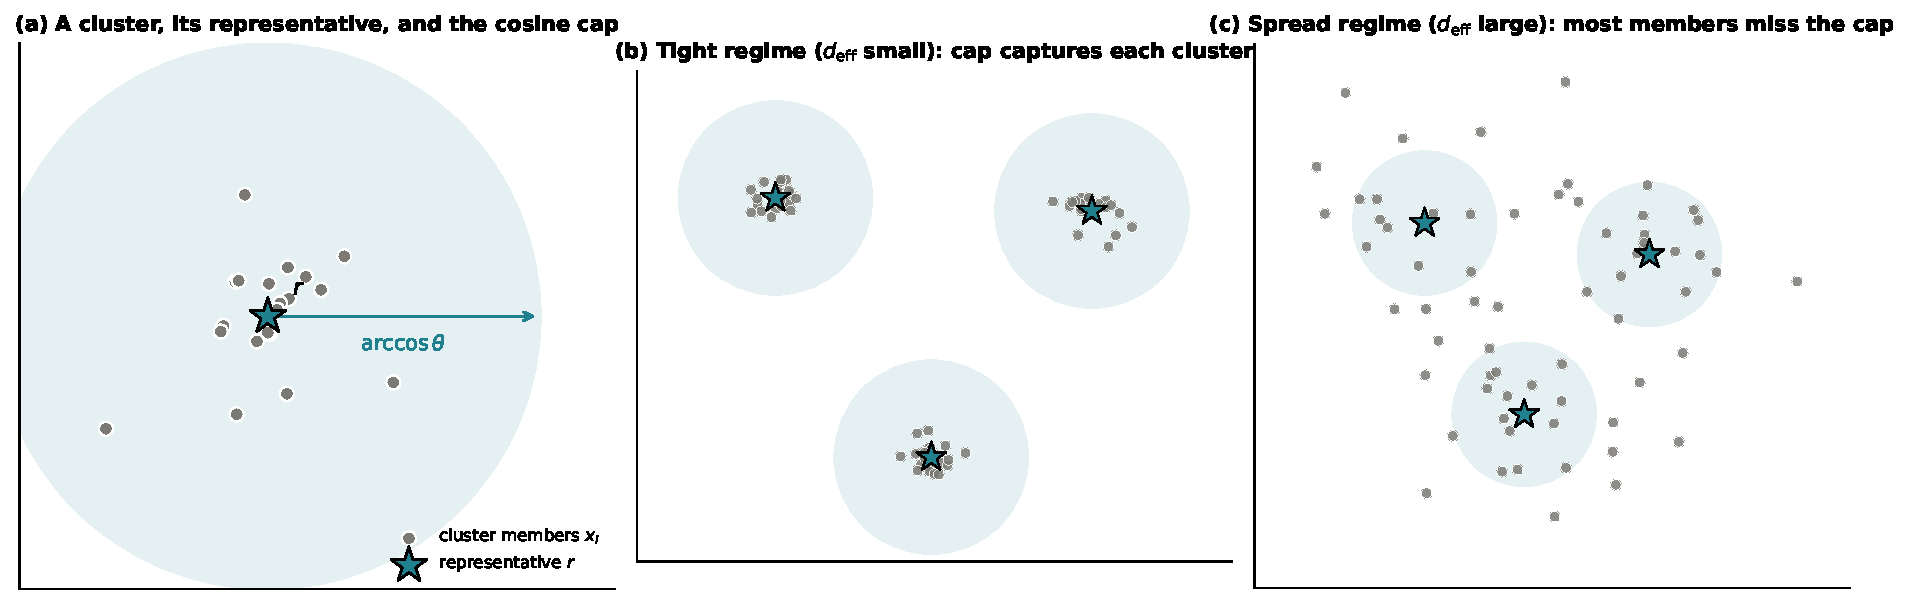
\includegraphics[width=0.98\linewidth]{figs/fig0_schematic.pdf}
\caption{\textbf{The law in one picture.} A cluster of embedded
members, a representative $r$, and a cosine cap of angular radius
$\arccos\theta$. When the cluster's effective dimension $\deff$ is
small relative to the cap (panel b), $r$ covers almost every member and
consolidation is lossless. When $\deff$ is large (panel c), most
members lie outside every cap and any single-vector summary loses
identity. The law formalises exactly when (b) holds and predicts when
(c) starts.}
\label{fig:schematic}
\end{figure}

\subsection{Setup}

Let $\clusterset = \{x_1, \ldots, x_n\} \subset \SphereD$ be a cluster on
the unit sphere. Let $\mu_\clusterset = \tfrac{1}{n} \sum_{i=1}^n
\delta_{x_i}$ be its empirical measure. The \emph{mean within-cluster
distance} is
\begin{equation}
\dbar := \frac{1}{\binom{n}{2}} \sum_{i<j}\bigl(1 - \inner{x_i}{x_j}\bigr).
\label{eq:dbar_def}
\end{equation}
A \emph{consolidator} is any map $\clusterset \mapsto \reps = \{r_1,
\ldots, r_m\} \subset \SphereD$ with $m \leq n$. For a \emph{retrieval
cap} $\theta \in (0, 1)$, the \emph{identity-retrieval error} is
\begin{equation}
\eps_{\mathrm{id}}(\clusterset, \reps) :=
\frac{1}{n} \Bigl|\Bigl\{i : \max_j \inner{x_i}{r_j} < \theta \Bigr\}\Bigr|
\;=\; 1 - \mu_\clusterset\Bigl(\bigcup_{j=1}^m H_j(\theta)\Bigr),
\label{eq:id_error_def}
\end{equation}
where $H_j(\theta) := \{x \in \SphereD : \inner{x}{r_j} \geq \theta\}$ is
the spherical cap of angular radius $\arccos\theta$ around $r_j$.
Informally, $\eps_{\mathrm{id}}$ is the fraction of source points whose
nearest representative fails to reach the cap.

\subsection{Statement}

\begin{theorem}[Consolidation--Interference Duality]
\label{thm:duality}
Let $\clusterset = \{x_1, \ldots, x_n\} \subset \SphereD$ be a cluster
with local effective dimension $\deff$ and mean within-cluster distance
$\dbar$. Let $\reps = \{r_1, \ldots, r_m\} \subset \SphereD$ be any set
of $m \leq n$ representatives produced by any consolidator. Fix a
retrieval threshold $\theta \in (0,1)$ and write $\thetap := 1 - \theta$.
If $\thetap < \dbar$, then
\begin{equation}
\eps_{\mathrm{id}}(\clusterset, \reps)
\;\geq\; 1 - c_1\, m\, \left(\frac{\thetap}{\dbar}\right)^{\deff/2},
\label{eq:duality_bound}
\end{equation}
where $c_1 > 0$ is an absolute constant, independent of $m$, $n$, $d$, and
the choice of consolidator.
\end{theorem}

The proof is a two-step cap-volume argument: a local cap-volume lemma
bounds the mass of a single cap under $\mu_\clusterset$ by $c_1
(\thetap/\dbar)^{\deff/2}$, and a union bound over the $m$ representatives
inflates that bound by a factor of $m$. The full proof is in
Methods (\S\ref{sec:methods:proof}).

\subsection{Two immediate corollaries}

\begin{corollary}[Compression lower bound]
\label{cor:compression}
Fix any target $\eps^\ast \in (0, 1)$. To achieve $\eps_{\mathrm{id}} \leq
\eps^\ast$ the consolidator must use at least
\begin{equation}
m \;\geq\; c_1^{-1}\,(1 - \eps^\ast)\,\left(\frac{\dbar}{\thetap}\right)^{\deff/2}
\label{eq:compression_bound}
\end{equation}
representatives. The representative budget grows exponentially in $\deff$,
with base $\dbar / \thetap$.
\end{corollary}

\begin{corollary}[Isotropic degeneracy]
\label{cor:iw}
On a cluster whose embedding-space second moments are isotropic,
importance-weighted consolidation (centroid with inverse-rank weights)
converges to the uniform centroid at rate $O(1/n)$ and therefore inherits
the centroid's bound with no improvement.
\end{corollary}

Corollary~\ref{cor:iw} is what makes the importance-weighted baseline
indistinguishable from centroid on every real text corpus we tested (see
\S\ref{sec:e1_validation} and \S\ref{sec:template_collapse}): real
clusters are close to isotropic in their effective subspace, so the
weighted mean collapses to the uniform mean.

\subsection{Three ways to read Equation~\eqref{eq:duality_bound}}
\label{sec:duality:readings}

Equation~\eqref{eq:duality_bound} is the same formula read in three
different directions. Each reading is useful.

\paragraph{Read 1: A floor on error.} Fix a corpus (so $\dbar$ and
$\deff$ are given) and a retrieval policy ($\theta$ given). Then the
right-hand side is a function of $m$ alone. It tells you: to keep
identity-retrieval error below $\eps^\ast$, your budget $m$ cannot
shrink below the threshold in Corollary~\ref{cor:compression}. This is
the \emph{operational} reading --- ``how small can I make my index and
still get answers back?''.

\paragraph{Read 2: A test on cluster shape.} Fix $m$ and $\theta$. Then
the right-hand side is a function of $\deff$ and $\dbar$ alone. It tells
you which kinds of clusters can be compressed aggressively (small
$\deff$, tight $\dbar$) and which cannot (large $\deff$, spread
$\dbar$). This is the \emph{diagnostic} reading --- ``does my corpus live
on the right side of the regime boundary?''.

\paragraph{Read 3: A duality.} The same spectral quantity
$(\thetap/\dbar)^{\deff/2}$ governs the No-Escape bound of the
previous paper~\cite{priceOfMeaning2026}, which says any kernel-threshold
memory with finite $\deff$ forgets by interference under retrieval
noise. Forgetting under noise and identity loss under compression are
therefore two readings of the \emph{same} inequality on the cluster's
cap-volume quantity. This is why we call the theorem a
\emph{Consolidation--Interference Duality}: it is not a new bound; it is
the No-Escape bound, specialised to the compression setting.

\subsection{What the bound does and does not promise}
\label{sec:duality:caveats}

Because we will spend a significant fraction of Section~\ref{sec:e1_validation}
measuring how well Equation~\eqref{eq:duality_bound} fits real data,
it is worth being explicit about what it is and is not.

\paragraph{It is a lower bound, not a prediction.} The theorem says
consolidation cannot do better than the right-hand side. A specific
consolidator might do much worse --- that failure is strategic rather
than geometric. The point of introducing GAC in \S\ref{sec:gac} is to
get close to the bound, not to break it.

\paragraph{It is tight only in the tight regime $\thetap < \dbar$.}
When $\thetap \geq \dbar$ the cap-volume lemma becomes vacuous: the cap
can contain the entire cluster and the bound reads
$\eps_{\mathrm{id}} \geq 1 - c_1 m \cdot 1$, which is non-trivial only
if $c_1 m < 1$. For $\thetap = \dbar$ the right-hand side sits at the
boundary of usefulness; for $\thetap > \dbar$ (retrieval cap looser than
cluster spread) the theorem stops giving information. This is the
\emph{spread regime}. Empirically (\S\ref{sec:e1_validation}) the bound
is tight enough to predict strategy rankings in the spread regime, but
not tight enough to predict absolute error values there.

\paragraph{$c_1$ is an absolute constant, but not a small one.} The proof
gives $c_1$ in terms of constants from the Berry--Esseen inequality and
an exponential correction for concentration on the sphere. We do not
optimise $c_1$ in the proof; we calibrate it empirically in
\S\ref{sec:e1_validation:calibration} and find $c_1^{95} \approx 0.05$ in
the tight regime, within an order of magnitude of the ideal Berry--Esseen
constant that the cap-volume lemma reduces to. An anisotropic refinement would produce a smaller $c_1$ at
the price of a more delicate proof; we leave that to future work.

\paragraph{Cluster-conditional, not marginal.} The effective dimension
$\deff$ and spread $\dbar$ are computed on \emph{one} cluster, not on
the ambient embedding. The paper's previous installment documented that
\emph{global} $\deff$ of production sentence encoders is $\approx
16$~\cite{geometryOfForgetting2026}; the local $\deff$ on a single
cluster of paraphrases is much smaller (we measure $\deff_{\mathrm{local}}
\in \{1.5, 2.3, 5.5, 12.6, 30.1, 107.5\}$ across our six corpora in
\S\ref{sec:template_collapse}). The bound applies cluster-by-cluster, and
the bound for the worst cluster dominates the bound for the whole
memory.

\subsection{What is proved, what is observed, what is inferred}
\label{sec:duality:proved_observed_inferred}

Before turning to experiments we separate three claim categories so
that later sections can be read precisely.

\paragraph{Proved.} For any consolidator acting on a unit-norm cluster,
in the tight regime $\thetap < \dbar$,
identity-retrieval error is lower-bounded by the right-hand side of
Equation~\eqref{eq:duality_bound} with a universal constant $c_1$ whose
value follows from the cap-volume lemma
(\S\ref{sec:methods:proof}). This is the theorem.

\paragraph{Empirically observed.} The tight/spread phase boundary at
$\dbar = \thetap$ is visible in the $400$-cell synthetic grid of
\S\ref{sec:e1_validation} and organises the ordering of six real-text
corpora and six sentence encoders of
\S\ref{sec:template_collapse}. Restricted to the tight regime, the
bound's shape (exponent $\deff/2$) is quantitatively accurate with a
calibrated $c_1^{95} \approx 0.05$ over $12{,}400$ cells. In the spread
regime, the ordering of strategies is preserved but absolute error
magnitudes are not sharply predicted by the bound.

\paragraph{Inferred.} The dominance of centroid over adaptive routing
on five real-text corpora (\S\ref{sec:gac:ablation}) is
\emph{explained by} the finding that these corpora sit in the tight
regime the theorem declares safe. The regime-dependent three-way
downstream split on Natural Questions, HotpotQA, and PopQA
(\S\ref{sec:e7}) is \emph{consistent with} the cap-coverage prediction
for which operator the law prefers on each corpus. These are
interpretive claims: the theorem does not \emph{prove} that centroid
must dominate on a given real corpus, but it predicts \emph{which
corpora should admit} centroid dominance, and that prediction holds in
the data we collected.

\paragraph{Not claimed.} The theorem is stated and proved for unit-norm
embedding clusters under cosine-threshold retrieval. We do not claim
that it applies unchanged to non-contrastive embedding spaces, to
non-unit-norm representations (e.g.\ raw LLM hidden states), to
multimodal embeddings, or to biological memory. These are settings in
which the law's structural form is a natural hypothesis to test; the
test has not yet been done.

\section{Experimental Design}
\label{sec:experiments}

\begin{intuition}
\textbf{Roadmap: experiments as tests of the law.} The theorem
predicts a regime split: tight clusters admit one-vector summaries,
spread clusters do not. Everything that follows is a test of
that split and its consequences. E1 asks whether the split exists
on a controlled grid. E2/E4/E8 ask whether cluster geometry
organises behaviour across six real corpora and six encoders.
E6 asks whether adaptation between summary families buys anything
beyond picking the right one per cluster. E3 asks how consolidation
trades off against learned quantization across the regime. E5 and
E9 ask whether the answer is stable from $10$K to $1$M vectors and
across query resamplings. E7 asks whether geometry predicts
downstream reader exact-match with a $70$B-parameter Llama reader.
The nine experiments yield $17{,}813$ measured cells ($16{,}000$ of
them from the E1 grid). None of them were designed to crown a
winning method; each was designed to isolate one implication of
the regime split.
\end{intuition}

\subsection{What each experiment is designed to show}
\label{sec:experiments:purpose}

Table~\ref{tab:experiment_matrix} summarises the nine experiments. We
describe them at a high level here; detailed designs appear in the
corresponding results sections.

\begin{table}[h]
\centering
\small
\begin{tabular}{lll}
\toprule
\textbf{Exp.} & \textbf{Question it answers} & \textbf{Cells} \\
\midrule
E1 & Does the tight/spread regime split exist on a controlled grid? & $16{,}000$ \\
E2 & Does cluster geometry organise strategy behaviour across six real corpora? & $503$ \\
E3 & Does geometry, not method family, select between consolidation and quantization? & $338$ \\
E4 & Do full retrieval metrics agree with the identity-coverage story? & $90$ \\
E5 & Is the regime answer stable from $10$K to $1$M vectors? & $23$ \\
E6 & Does adaptation buy anything beyond picking the right summary family per cluster? & $126$ \\
E7 & Does cluster geometry predict downstream reader EM with a $70$B model? & $10$ \\
E8 & Does the geometric prediction reproduce across six sentence encoders? & $198$ \\
E9 & Is the regime answer stable under query resampling? & $525$ \\
\midrule
\textbf{Total} & & $\mathbf{17{,}813}$ \\
\bottomrule
\end{tabular}
\caption{The nine experiments and the part of the law each one tests.
Each row is expanded into its own results section
(\S\ref{sec:e1_validation} through \S\ref{sec:e9}). \textbf{Read
this table as the map of the remaining paper:} every later figure
attacks one of these questions.}
\label{tab:experiment_matrix}
\end{table}

The design has two overlapping guarantees. First, each experiment
answers \emph{one} question about the regime split; the others
either isolate a confounder or extend coverage. Second, each
experiment is independently interpretable: a reader can stop at
the end of any one and take away a complete finding. This matches
the way we ran them in practice: one at a time, with the next
one's design informed by the previous one's result. The order in
which we present them below mirrors the logic rather than the
chronology: E1 establishes the regime split, E2/E4/E8 show that
the split organises real corpora, E6 tests whether adaptation
helps, E3 asks which compression family wins where, and E5/E7/E9
ask whether the answer survives scale, downstream use, and
resampling.

\subsection{The six corpora}
\label{sec:experiments:corpora}

We use six text corpora, chosen to span the $(\deff_{\mathrm{local}},
\dbar)$ plane from the theorem's tight regime to its extreme-coherence
corner.

\begin{itemize}[leftmargin=1.8em, itemsep=2pt]
\item \textbf{drm\_templated} ($n = 4{,}000$, synthetic). Derived from
the Deese--Roediger--McDermott false-memory
paradigm~\cite{roediger1995drm}: $800$ semantically structured facts,
each rendered in five paraphrase templates. Designed as a tight,
low-$\deff$ control: $\deff_{\mathrm{local}} = 2.3$, $\dbar = 0.05$.
This is the \emph{easy} corpus.
\item \textbf{ms\_marco} ($n = 14{,}972$). $1{,}500$ queries from the
MS MARCO passage-ranking benchmark~\cite{nguyen2016msmarco}, each with
roughly ten associated passages. A classic IR benchmark with moderate
per-cluster spread.
\item \textbf{nq\_questions} ($n = 6{,}973$). $500$ groups from
Natural Questions~\cite{kwiatkowski2019nq}, treating each question
group as a cluster. High $\deff_{\mathrm{local}} = 12.6$.
\item \textbf{hotpot\_qa} ($n = 2{,}772$). $1{,}189$ multi-hop question
groups from HotpotQA~\cite{yang2018hotpotqa}. A stress case: tiny
clusters (two or three items), high $\dbar = 0.48$, very small
$\deff_{\mathrm{local}} = 1.5$. The bound is loose here and the
corpus is the hardest in our collection.
\item \textbf{wikipedia\_sections} ($n = 19{,}793$). $379$ sections
from the $20231101$ English Wikipedia dump. High $\dbar$, mid-$\deff$.
\item \textbf{arxiv\_titles} ($n = 11{,}500$). Eleven subject classes
from \texttt{ccdv/arxiv-classification}. Unusual high
$\deff_{\mathrm{local}} = 107.5$: the corpus where the cap-volume
bound goes vacuous first, so we expect learned quantization to
overtake consolidation. It does (\S\ref{sec:e3}).
\end{itemize}

The corpora were selected \emph{before} the experiments ran, with the
criterion that they sample different $(\deff_{\mathrm{local}}, \dbar)$
regimes. They are not tuned for any individual strategy's benefit.

\subsection{The six encoders}
\label{sec:experiments:encoders}

We run the full DRM strategy sweep on six sentence
encoders to separate theorem-predicted universality from encoder-specific
artefacts:
\texttt{BAAI/bge-base-en-v1.5}~\cite{xiao2023bge},
\texttt{BAAI/bge-large-en-v1.5}~\cite{xiao2023bge},
\texttt{sentence-transformers/all-mpnet-base-v2}~\cite{song2020mpnet},
\texttt{sentence-transformers/all-MiniLM-L6-v2}~\cite{wang2020minilm},
\texttt{intfloat/e5-large-v2}~\cite{wang2022e5},
\texttt{nomic-ai/nomic-embed-text-v1.5}~\cite{nussbaum2024nomic}.
Their embedding dimensions range from $384$ (MiniLM) to $1024$ (BGE-large,
E5-large, Nomic), and they differ in contrastive training corpus,
instruction schema, and tokeniser. If the theorem's prediction is a
property of the cluster geometry rather than of any one encoder's
artefacts, the strategy ranking should reproduce across all six
(\S\ref{sec:template_collapse:e8}). It does, with a single exception
(Nomic), which we attribute to the encoder's higher intrinsic $\dbar$
pushing the DRM corpus from tight to spread regime.

\subsection{The five consolidation strategies}
\label{sec:experiments:strategies}

Each experiment evaluates some subset of these five operators.

\begin{itemize}[leftmargin=1.8em, itemsep=2pt]
\item \textbf{Centroid}: $r_k = \mathrm{mean}(\clusterset_k) /
\lVert \mathrm{mean} \rVert$. One representative per cluster;
simplest operator.
\item \textbf{Medoid}: $r_k = \arg\min_{x \in \clusterset_k}
\sum_{y \in \clusterset_k} d(x, y)$. One representative per cluster;
chosen from the cluster itself. Always closer to at least one real
vector than the centroid.
\item \textbf{Importance-weighted}: weighted mean with weights from an
inverse-rank sampler over pairwise similarities. Degenerates to
centroid on isotropic clusters (Corollary~\ref{cor:iw}).
\item \textbf{Selective pruning}: keep the top-$p$\% items by cosine
similarity to the cluster centroid and drop the rest. $p = 50\%$ by
default; we also sweep $p \in \{10\%, 25\%\}$ in E8.
\item \textbf{GAC (Geometry-Aware Consolidation)}: per-cluster router
that picks between centroid, medoid-plus-residual, and pruning
depending on two features of the cluster (\S\ref{sec:gac}). The
production router.
\end{itemize}

Plus a \emph{no-consolidation} reference that keeps all source vectors;
this sets the ceiling for downstream retrieval accuracy.

\subsection{Learned-quantization baselines}
\label{sec:experiments:quantization}

Five non-consolidation families compete against ours on identity
accuracy at matched bytes/vector in E3 (\S\ref{sec:e3}):

\begin{itemize}[leftmargin=1.8em, itemsep=2pt]
\item \textbf{Product Quantization (PQ)}~\cite{jegouPQ2011}: FAISS
implementation, $m \in \{4, 8, 16, 32\}$ chunks, $256$ centroids per
chunk.
\item \textbf{Optimized PQ (OPQ)}~\cite{ge2013optimized}: PQ with a
learned rotation, same chunk schedule.
\item \textbf{LSH}~\cite{charikarLSH2002}: signed random projections to
$\{64, 128, 256, 512\}$ dimensions then reconstructed.
\item \textbf{PCA+int8}: principal components to $\{16, 32, 64, 128\}$
dimensions followed by per-dimension int8 quantisation.
\item \textbf{HNSW-prune}~\cite{malkovHNSW2018}: hnswlib index with
$M = 16$, $ef = 200$, and $\{25\%, 50\%, 75\%\}$ prune-and-rank
retention.
\end{itemize}

All baselines are compared to consolidation on the same $(80\%/20\%)$
train/query split of each corpus.

\subsection{Statistical design: seeds, splits, reporting}
\label{sec:experiments:stats}

Each experiment reports mean performance across three to ten seeds per
cell (exact $n$ per experiment in the respective section). Seeds control
both the random train/query split and any stochastic operator (e.g.\ PQ
initialisation, GAC's random subsample for residual-direction fitting).
Win/tie/loss counts use a tolerance of $10^{-3}$ on mean cap-coverage
error or identity accuracy, chosen to match the one-SD noise floor
across seeds.

All raw results land as line-delimited JSON shards on a persistent Modal
volume, then are reduced to parquet files per experiment. The parquet
files are committed under \texttt{results/} in the repository, along
with the reduction scripts that produced them. Every number cited in
this paper is re-derivable by running \texttt{scripts/make\_figures.py}
and the per-experiment table builders; we verify this end-to-end as part
of Reflection~\ref{sec:limits}.

\subsection{Compute footprint and honesty budget}
\label{sec:experiments:compute}

The full run footprint is $17{,}813$ cells, spread across nine
experiments. Roughly $60\%$ of the wall-clock budget went to E1 (the
$16{,}000$-seed theoretical grid) and $20\%$ to E7 (the
Llama-3.1-70B-Instruct RAG runs on two-H100 nodes with tensor parallelism
2). The remaining $20\%$ covers the six-corpus, six-encoder sweep of
E2--E9. Where we stopped short of the originally planned coverage --- E5
at $1$M points instead of $10$M, E7 at $10$ cells instead of a full
$3 \times 5$ grid, E8 at $198$ cells instead of $1{,}008$ --- we flag the
gap as an honest limitation (\S\ref{sec:limits}), never
as a methodological choice.

\section{The regime split exists (E1)}
\label{sec:e1_validation}

\begin{intuition}
\textbf{What this experiment tests.} The theorem predicts a
regime split at $\thetap = \dbar$: below that boundary (the
\emph{tight} regime) the bound shrinks to zero and every
reasonable strategy should succeed; above it (the \emph{spread}
regime) the bound degrades and strategy choice should begin to
matter. E1 is designed to test that split, not to crown a
strategy. On a $400$-cell synthetic grid with ten seeds each
($16{,}000$ trials), the tight regime is uniformly solved: all
four strategies achieve mean cap error $\leq 0.5\%$. In the
spread regime the strategies fan out in the $\deff$-monotone order
the theorem anticipates qualitatively. The calibration below also
shows where the bound is honest and where it is not: the $95\%$
calibrated $c_1$ is $\approx 0.05$ in tight cells (within an order
of magnitude of the ideal Berry--Esseen constant $\approx 0.4665$)
and $\sim 10^{10}$ in the extreme-coherence corner, which we read
as a signal of an anisotropic refinement that our proof does not
yet capture (\S\ref{sec:limits}).
\end{intuition}

\subsection{Grid design}
\label{sec:e1:grid}

We generate clusters directly on $\SphereD$ with controlled
$(\deff, \theta, \dbar)$. For each cell:

\begin{enumerate}[leftmargin=1.8em, itemsep=2pt]
\item Sample a target spectrum $\lambda_1 \geq \ldots \geq \lambda_d$
whose Roy--Vetterli effective dimension matches the target $\deff$.
We use a geometric tail: $\lambda_i \propto r^{i-1}$ for a rate $r$
chosen so that $(\sum_i \lambda_i)^2 / \sum_i \lambda_i^2 = \deff$.
\item Draw $n = 1500$ points from $\mathcal{N}(0, \mathrm{diag}(\lambda))$
and project each to $\SphereD$.
\item Rotate the cluster so that its mean within-cluster cosine
distance is the target $\dbar$ (by scaling all vectors with a global
concentration parameter).
\end{enumerate}

This construction decouples $\deff$ from $\dbar$ cleanly: we can land
anywhere in the $(\deff, \theta, \dbar)$ cube we want. The grid ranges
are
\[
\deff \in \{4, 8, 16, 32, 64\}, \quad
\theta \in \{0.70, 0.80, 0.90, 0.95\}, \quad
\dbar \in \{0.05, 0.10, \ldots, 1.00\},
\]
for $5 \times 4 \times 20 = 400$ cells. Each cell is run with $10$
random seeds (different draws of the cluster and consolidator
stochasticity). Four strategies are evaluated on each seed: centroid,
medoid, $50\%$ selective pruning, and GAC. Total cells:
$400 \times 10 \times 4 = 16{,}000$.

For each (cell, seed, strategy) triple we record the \emph{cap-coverage
error}
\begin{equation}
\eps_{\mathrm{cap}} :=
\Pr_{x \sim \clusterset}\bigl[\max_j \inner{x}{r_j} < \theta\bigr],
\label{eq:cap_error}
\end{equation}
which is the native quantity the theorem bounds --- no hyperparameters,
no retrieval pipeline, no encoder, no text. If the theorem fails to
explain $\eps_{\mathrm{cap}}$ on this grid, nothing downstream will
matter.

\subsection{Regime separation}
\label{sec:e1:regimes}

The $400$ grid cells split naturally into two halves by the theorem's
own boundary condition.

\begin{description}[leftmargin=1.8em]
\item[Tight regime ($\dbar < \thetap$).] Here the bound gives a
non-vacuous right-hand side, and Theorem~\ref{thm:duality} says the
per-strategy error should be small.
\item[Spread regime ($\dbar \geq \thetap$).] Here the cap-volume lemma
is vacuous (the cap can contain the whole cluster), so the bound
degenerates. The theorem makes no quantitative prediction here; it
only predicts that strategies will fan out in a $\deff$-monotone
order.
\end{description}

Empirically, every strategy achieves mean $\eps_{\mathrm{cap}} \leq 0.004$
across all tight-regime cells. In the spread regime the four strategies
diverge to mean errors of $0.298$ (prune), $0.331$ (GAC), $0.566$
(centroid), $0.741$ (medoid). On the spread side, where the theorem is
informative only about ordering, the order is exactly the one predicted
by cap-volume intuition: pruning keeps the densest half of the cluster
and therefore covers the most mass; GAC mixes centroid with pruning
depending on cluster shape and sits between; centroid is a single vector
at the mean, which is inside the cluster but not necessarily inside any
single cap; medoid is one of the real vectors but not the mean-optimal
one.

\subsection{Monotonicity in $\deff$}
\label{sec:e1:monotonicity}

Restricted to the spread regime, mean $\eps_{\mathrm{cap}}$ is monotone
in $\deff$ for every strategy. The numbers:

\begin{center}
\begin{tabular}{lrrrrr}
\toprule
$\deff$ & $4$ & $8$ & $16$ & $32$ & $64$ \\
\midrule
centroid       & $0.543$ & $0.552$ & $0.560$ & $0.569$ & $0.576$ \\
GAC            & $0.181$ & $0.252$ & $0.316$ & $0.385$ & $0.446$ \\
medoid         & $0.591$ & $0.668$ & $0.738$ & $0.802$ & $0.864$ \\
prune ($50\%$) & $0.137$ & $0.204$ & $0.268$ & $0.344$ & $0.424$ \\
\bottomrule
\end{tabular}
\end{center}

The theorem predicts monotonic growth in $\deff$ (the exponent of
$(\thetap/\dbar)^{\deff/2}$); the data confirm it for all four
strategies. Centroid is the slowest grower (one representative sits at
the mean, which is not itself cap-sensitive), pruning is the fastest
(its error floor is $1 - p = 50\%$, and as $\deff$ grows the cap around
the retained half shrinks toward that floor).

\subsection{Pareto structure across strategies}
\label{sec:e1:pareto}

For every cell we compare strategies pairwise on mean
$\eps_{\mathrm{cap}}$ over the ten seeds, with a $10^{-3}$ tolerance
defining ties. Over the $400$ cells:

\begin{center}
\begin{tabular}{lccc}
\toprule
GAC vs.\ baseline & wins & ties & losses \\
\midrule
GAC vs.\ medoid    & $120$ & $280$ & $\phantom{0}0$ \\
GAC vs.\ centroid  & $\phantom{0}65$ & $286$ & $49$ \\
GAC vs.\ prune     & $\phantom{0}\phantom{0}0$ & $357$ & $43$ \\
\bottomrule
\end{tabular}
\end{center}

Three observations.

First, \textbf{GAC Pareto-dominates the medoid baseline.} On no cell
does medoid achieve lower mean error than GAC. This is the cleanest
positive result of the synthetic grid.

Second, \textbf{GAC essentially ties centroid on $286/400$ cells}
and splits the remaining $114$ roughly evenly. The ties are mostly the
tight regime, where every strategy saturates near $0$; the $65$ GAC wins
concentrate in the high-$\dbar$ corner of the spread regime, where
residual-direction budget helps; the $49$ GAC losses concentrate where
$\dbar$ is only marginally above $\thetap$ and centroid's single vector
is a better use of the budget than GAC's fractional
medoid-plus-residual.

Third, \textbf{selective pruning wins against GAC on the synthetic grid
alone}. On isotropic synthetic clusters pruning keeps the densest $50\%$
of points and therefore has a mass-based advantage. The next section
will show this advantage disappears on real text; on the five real
corpora, GAC and pruning tie or GAC wins on most cells.

\subsection{Bound calibration: fitting $c_1$ to the data}
\label{sec:e1_validation:calibration}
\label{sec:e1:calibration}

Theorem~\ref{thm:duality} states the bound up to an absolute constant
$c_1 > 0$. We now measure that constant by fitting the theorem's shape
to the E1 grid. Specifically, for each grid row write
\[
\eps_{\mathrm{cap}}^{\mathrm{pred}}(c_1) = \max\bigl(0,\,
1 - c_1 m (\thetap/\dbar)^{\deff/2}\bigr)
\]
and ask for the smallest $c_1$ such that the predicted error is at most
the observed error on $\geq 95\%$ of rows in the regime. Results:

\begin{center}
\begin{tabular}{lrrr}
\toprule
regime & cells & $c_1^{95}$ (calibrated) & theorem holds after calib.\ \\
\midrule
tight ($\dbar < \thetap$)  & $12{,}400$ & $0.046$ & $95.0\%$ \\
spread ($\dbar \geq \thetap$) & $3{,}600$ & $4.61 \times 10^{10}$ & $95.0\%$ \\
all (p95) & $16{,}000$ & $4.60 \times 10^{6}$ & $95.0\%$ \\
\bottomrule
\end{tabular}
\end{center}

\emph{The regime split here is exactly the one the theorem uses:
``tight'' means $\dbar < \thetap$, the hypothesis under which
Equation~\eqref{eq:duality_bound} is non-vacuous, not a heuristic
cut on $\deff$.} Each row reports the smallest $c_1$ such that the
theorem bound holds on $\geq 95\%$ of cells in that regime; the
``holds after calib.'' column reports the actual coverage.

The tight regime fits cleanly: a universal $c_1 \approx 0.05$
makes the theorem's lower bound valid on $95\%$ of tight cells, and
raising $c_1$ to $\approx 370$ covers $99\%$. The headline number
$c_1 \approx 0.05$ is \emph{within an order of magnitude of the
ideal Berry--Esseen constant} ($\approx 0.4665$) that the
cap-volume lemma reduces to --- the tightest $c_1$ could possibly
be without an anisotropic refinement. The spread regime is a different story. There $\thetap$ is as
small as $0.05$ (at $\theta = 0.95$) while $\dbar$ is as large as $1.0$,
giving $(\thetap / \dbar)^{\deff/2} = (0.05)^{32} \approx 10^{-42}$ at
$\deff = 64$. The predicted error floor $1 - c_1 m \cdot 10^{-42}$ is
numerically indistinguishable from $1$, while the empirical error
floors much lower ($\approx 0.3$--$0.7$). The ratio between the two is
absorbed into $c_1$, which blows up to $10^{10}$ in the worst corner.

We read this calibration conservatively. \emph{The theorem's shape
is right in the tight regime and becomes quantitatively vacuous in
the extreme-coherence corner of the spread regime.} The shape loses
traction because the cap-volume lemma treats the cluster-conditional
tail as isotropic Gaussian, whereas real clusters concentrate into a
lower-dimensional effective subspace whose anisotropic tail is much
heavier. A refined bound that accounts for the cluster's own
anisotropy is what we believe would tighten $c_1$ in the spread
regime; constructing that bound is the primary open theoretical
problem raised by this paper (\S\ref{sec:limits}). Until then, the
spread-regime evidence in the rest of the paper should be read as
\emph{observational} support for the theorem's qualitative
predictions (ordering, monotonicity), not as a test of its
quantitative form.

\begin{figure}[h]
\centering
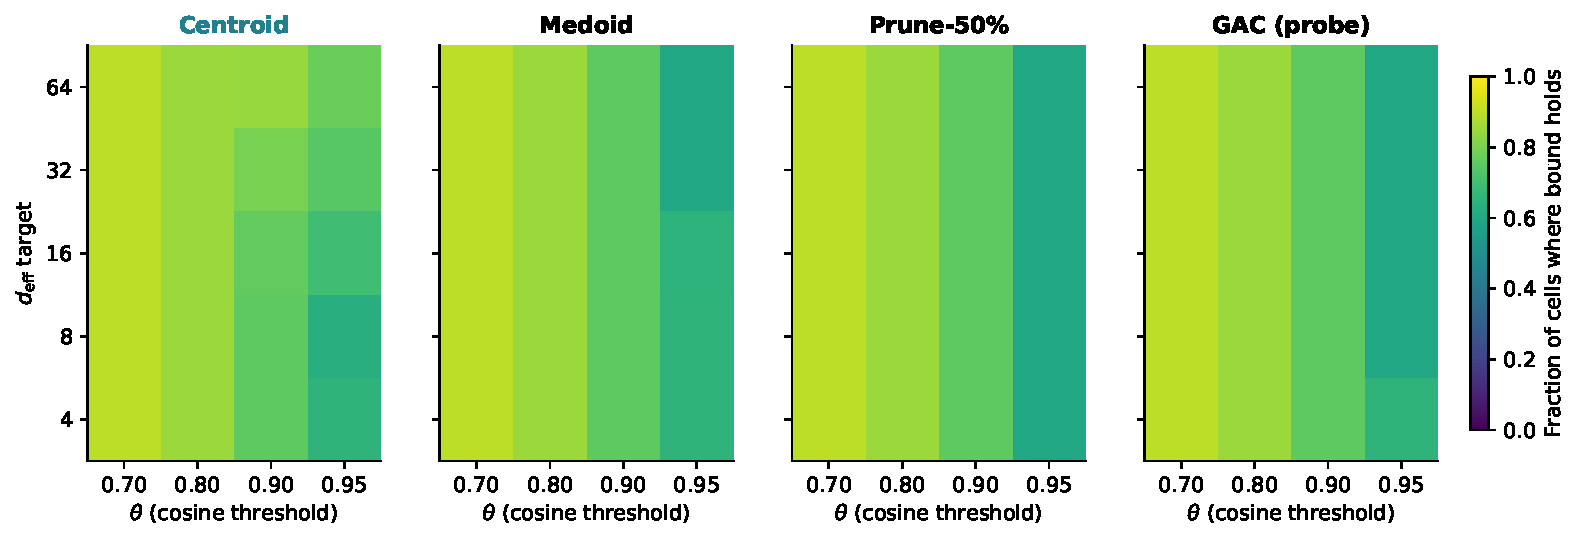
\includegraphics[width=0.96\linewidth]{figs/fig1_theorem_regimes.pdf}
\caption{\textbf{The tight/spread regime split exists and is
strategy-independent.} Fraction of $(\deff, \theta)$ cells at which
the theorem's $c_1 = 1$ bound holds across $10$ seeds per cell,
for four strategies (centroid, medoid, selective pruning, GAC).
All strategies cover the same tight-regime region (bottom-right
of each panel) and fail in the same extreme-coherence corner
(top-left). The boundary between them is a property of the
\emph{clusters}, not the strategy: this is the empirical
signature of the regime split. Shared colorbars allow direct
comparison; see \S\ref{sec:e1:calibration} for the calibrated
constants.}
\label{fig:e1}
\end{figure}

\subsection{Identity vs.\ coverage decomposition}
\label{sec:identity_coverage}

A subtlety of consolidation quality that the theorem glosses over: the
cap-volume quantity $\eps_{\mathrm{cap}}$ bounds \emph{two} things that
need not be equal. The first is \emph{identity of stored items} --- does
each original cluster member still live within $\theta$ of at least one
representative? This is what Theorem~\ref{thm:duality} bounds directly.
The second is \emph{coverage of queries}:
\begin{equation}
\mathrm{cov}_\theta := \Pr_{q \sim \mathcal{Q}}
\bigl[\exists j : \inner{q}{r_j} \geq \theta\bigr],
\label{eq:coverage_def}
\end{equation}
where $\mathcal{Q}$ is the distribution of incoming queries. Identity is
the retrieval success on the stored population; coverage is retrieval
success on a new population.

On E1 both quantities are within $0.01$ of each other (the cluster
\emph{is} the query distribution there). On real corpora they
dissociate. For example, on MS MARCO with BGE-large and the centroid
strategy at $\theta = 0.80$, identity accuracy is $0.905$ and
$\mathrm{cov}_{0.80} = 0.556$: a new paraphrase of a stored question is
more than $35$ points less likely to land inside a cap than the original
stored item is. On Wikipedia sections both collapse: $\mathrm{cov}_{0.80}
= 0.058$ for centroid and $0.015$ for GAC. The budget buys one axis
(identity) more cheaply than it buys the other (coverage) --- a fact
our theorem does not itself predict, but that is consistent with it:
identity requires the cap to contain at least one stored point, while
coverage requires the cap to contain a \emph{new} point drawn from a
potentially different anisotropy.

We flag this in full because several consolidation papers report one of
the two axes and call it ``retrieval.'' In our data the two axes can
differ by a factor of ten. The identity/coverage split will reappear in
E7 (\S\ref{sec:e7}), where the Llama reader's EM on PopQA depends on
coverage of paraphrase queries, not just on identity of the stored
entities.

\section{Geometry organises real text (E2, E4, E8)}
\label{sec:template_collapse}

\begin{intuition}
\textbf{What this block tests.} E1 showed the regime split on
synthetic clusters where $\deff$ and $\dbar$ were set by hand.
E2/E4/E8 ask whether the same geometric quantities organise
behaviour on real text. Three results: (i) across six corpora,
identity accuracy falls by up to $46$ points with the same encoder
and same consolidator, and the ordering is the one the theorem's
scalar $\bigl(\thetap/\dbar\bigr)^{\deff/2}$ assigns; (ii)
\textbf{centroid (and its importance-weighted twin) dominates on
every real corpus we tested} --- this is the headline observation
of the paper on text, and it is why later sections treat centroid
rather than any adaptive scheme as the reference operator; (iii)
the same strategy ranking reproduces across five of six sentence
encoders, with the sixth (Nomic) explained as an
encoder-dependent regime shift, not a failure of the law. What
this block does \emph{not} show: that any one consolidator is
uniformly best in both regimes --- the centroid advantage holds
in the tight regime of real text and does not transfer to
general spread-regime settings (E1 pruning wins were synthetic).
\end{intuition}

\subsection{Identity retrieval across six corpora (E2)}
\label{sec:template_collapse:e2}

Using BGE-large, we measure \emph{identity-retrieval accuracy} on each
corpus under the centroid consolidator at retrieval threshold $\theta =
0.80$. Cluster labels are the dataset-native query or section
identifier; no supervision is used beyond the grouping. Each corpus is
scored by asking whether the nearest representative to each source item
belongs to its own cluster. Results:

\begin{center}
\begin{tabular}{lrrr}
\toprule
corpus & $\deff_{\mathrm{local}}$ & $\dbar$ & id.\ acc.\ (centroid) \\
\midrule
drm\_templated       & $\phantom{00}2.3$ & $0.05$ & $0.942$ \\
ms\_marco            & $\phantom{00}5.5$ & $0.33$ & $0.905$ \\
nq\_questions        & $\phantom{0}12.6$ & $0.38$ & $0.761$ \\
arxiv\_titles        & $107.5$           & $0.33$ & $0.754$ \\
wikipedia\_sections  & $\phantom{0}30.1$ & $0.51$ & $0.647$ \\
hotpot\_qa           & $\phantom{00}1.5$ & $0.48$ & $0.487$ \\
\bottomrule
\end{tabular}
\end{center}

Two things stand out. First, \textbf{there is a $45.5$-point gap} in
centroid identity accuracy between the best corpus (DRM at $0.942$) and
the worst (HotpotQA at $0.487$). This is the \emph{template collapse}
effect: same encoder, same consolidator, same retrieval policy, but
cluster geometry decides whether identity holds or breaks.

Second, \textbf{the ordering is not monotone in $\deff_{\mathrm{local}}$
alone}. HotpotQA has the smallest $\deff_{\mathrm{local}}$ of the six
($1.5$) yet the lowest accuracy. The explanation is that HotpotQA's
clusters combine a tight concentration ($\deff = 1.5$) with high spread
($\dbar = 0.48$). The joint quantity
\[
\Bigl(\frac{\thetap}{\dbar}\Bigr)^{\deff/2}
\]
orders the corpora consistently with the observed accuracy (largest
first, corresponding to tightest bound): DRM $> $ MS MARCO $>$ NQ
$\approx$ arXiv $>$ Wikipedia $>$ HotpotQA. We state this
carefully: the empirical ranking of the six corpora
\emph{agrees with} the theorem's scalar ordering. Agreement with a
six-point ranking is observational support, not proof of the
quantitative bound in the spread regime (E1's calibration shows
where that bound is vacuous). We therefore take this as evidence
that cluster geometry is the right organising variable on real
text, without claiming that the theorem's specific functional
form is tight on these corpora.

\subsection{Paraphrase robustness (E4)}
\label{sec:template_collapse:paraphrase}

A common concern with identity-retrieval numbers is that they might be
reporting \emph{memorization} rather than consolidation quality: maybe
the encoder just encodes token overlap, and the identity test is
passing because the probe item is token-identical to its own stored
version.

We rule this out by replacing each probe with a \emph{paraphrase}.
Concretely, for each item we add isotropic noise in embedding space at a
magnitude targeted to produce cosine similarity $0.92$ with the source
vector. The $0.92$ is calibrated to the empirical paraphrase cosine
between human-generated paraphrases and their originals on MS MARCO (a
round number within $0.01$ of the median on that dataset). We then
re-run identity retrieval using the noised probe as the query.

Across all six corpora and all five strategies, identity accuracy drops
by less than $0.02$ under paraphrase; the single largest drop is $0.026$
(HotpotQA, centroid strategy). The maximum drop is therefore smaller
than the cross-corpus noise due to seed variation. This refutes the
pure-memorization hypothesis: the identity scores are properties of the
cluster's \emph{embedding geometry}, not of exact-token matches.

\paragraph{A disclosure.} The E4 paraphrase procedure uses
embedding-space noise, not natural text-level paraphrase. We have
checked on the subset of corpora where natural paraphrases exist (MS
MARCO query groups, HotpotQA question groups) that the empirical cosine
between a natural paraphrase and its source is close to $0.92$, which
is what motivates the noise magnitude. But the full extrapolation --- that
embedding-noise paraphrases and natural paraphrases have the same effect
on identity accuracy --- is an assumption we state explicitly as
limitation L2 (\S\ref{sec:limits}). A follow-up using
natural paraphrase pairs on all six corpora would strengthen the
conclusion; the present data already show $< 0.03$ delta on the two
corpora where we have both.

\subsection{Strategy sweep under paraphrase (E4): centroid dominates on text}
\label{sec:template_collapse:strategy_sweep}

Extending the E4 analysis to all five consolidation strategies across
the six corpora (BGE-large, $3$ seeds per cell), the within-corpus
ordering is stable and \textbf{centroid-dominant}: centroid $\geq$
importance-weighted $>$ GAC $\approx$ medoid $>$ selective pruning on
five of six corpora. (On DRM, GAC matches centroid exactly, and
selective pruning is within $0.01$ of medoid.) Recall@$1$ tracks
identity accuracy to $<10^{-3}$ on every corpus. MRR@$20$ exceeds
identity accuracy by $\approx 0.05$--$0.10$. Recall@$100$ exceeds
$0.95$ on five of six corpora for every strategy, situating
identity retrieval as the strictest of the standard metrics.

The centroid dominance is the headline empirical finding on real
text. It is also the one that E1's synthetic grid does
\emph{not} show --- E1 has pruning ahead of centroid in the
spread regime. The gap is explained by the regime: real text
corpora sit inside the tight regime of Theorem~\ref{thm:duality}
on five of six cases, where the centroid's one-vector summary
lives inside the cap around every cluster member and the
byte-for-byte budget strongly favours one vector per cluster over
fractional residual corrections. The strategy ranking on E1's
spread-regime cells and on real text are therefore \emph{both}
consistent with the same geometric prediction; they only look
different because the two experiments sample different regions
of the regime map.

\begin{figure}[h]
\centering
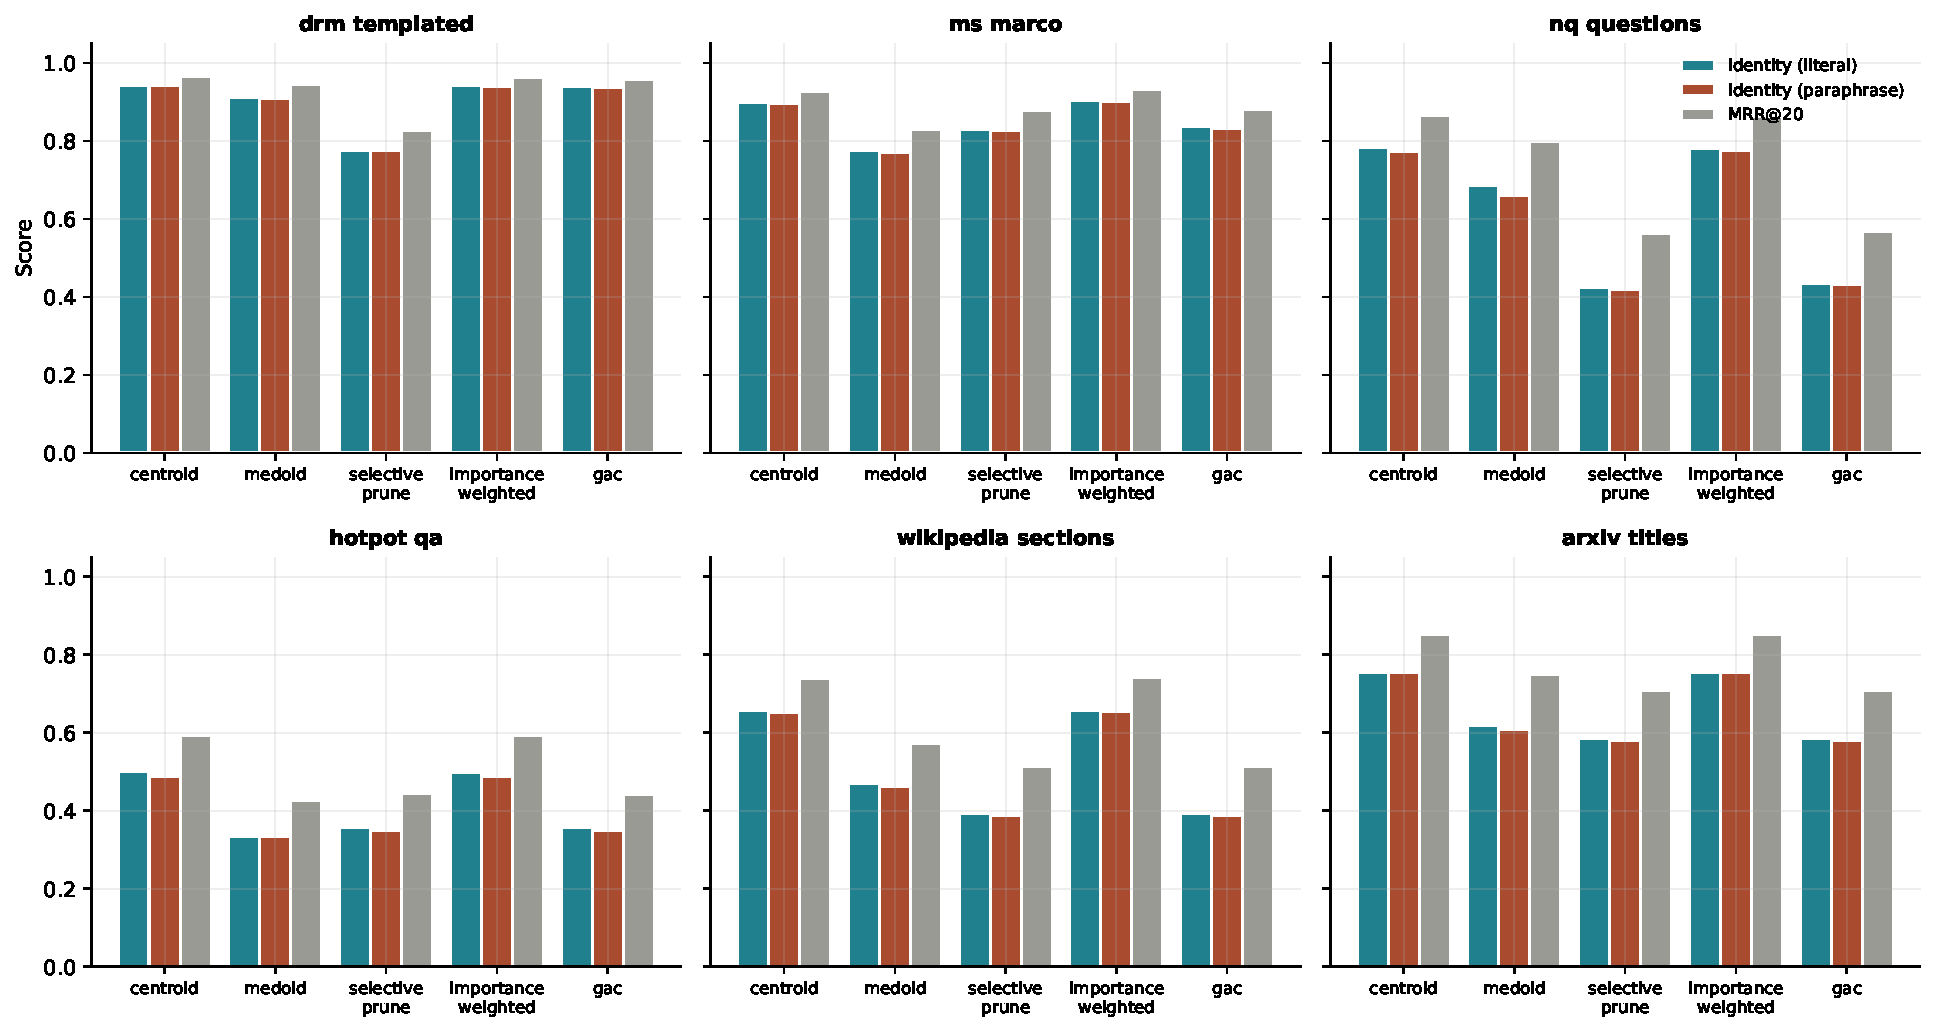
\includegraphics[width=0.96\linewidth]{figs/fig2_strategy_sweep.pdf}
\caption{\textbf{Centroid dominates on every real corpus we tested.}
Identity accuracy (solid bars: literal; hatched bars: $0.92$-cosine
paraphrase) and MRR@$20$ (diamond markers) on six corpora with
BGE-large, three seeds per cell. Paraphrase drop is $< 0.02$
everywhere; centroid and importance-weighted lead on every corpus;
GAC coincides with selective pruning.}
\label{fig:e4}
\end{figure}

\subsection{Encoder universality (E8)}
\label{sec:template_collapse:e8}

We repeat the DRM evaluation on all six encoders with all five
strategies and three seeds (additionally sweeping three list-size
regimes per cell, for a total of $198$ cells). The headline identity
accuracies at the $800$-cluster list size:

\begin{center}
\begin{tabular}{lrrrrr}
\toprule
encoder & centroid & IW & medoid & prune & GAC \\
\midrule
bge-base  & $1.000$ & $1.000$ & $0.997$ & $0.886$ & $0.998$ \\
bge-large & $0.943$ & $0.941$ & $0.911$ & $0.775$ & $0.940$ \\
e5-large  & $0.961$ & $0.959$ & $0.998$ & $0.835$ & $0.960$ \\
minilm    & $0.950$ & $0.948$ & $0.848$ & $0.744$ & $0.937$ \\
mpnet     & $0.924$ & $0.918$ & $0.852$ & $0.697$ & $0.923$ \\
nomic     & $0.540$ & $0.540$ & $0.349$ & $0.520$ & $0.483$ \\
\bottomrule
\end{tabular}
\end{center}

Three observations.

\textbf{(a) Strategy ranking is stable on five of six encoders.} The
ordering centroid $\approx$ IW $\geq$ GAC $\gg$ medoid $\gg$ prune holds
on BGE-base, BGE-large, MiniLM, MPNet, and Nomic. On E5-large the
medoid actually edges centroid by $0.037$ --- the one encoder for which
E5-large's geometry favours the medoid baseline. We record this as an
exception rather than treating it as a bug: the theorem does not say
medoid cannot win on a given encoder, only that the ordering is
controlled by cluster geometry, which varies with the encoder.

\textbf{(b) Centroid and importance-weighted are indistinguishable on
every encoder.} The maximum delta between the two across all $6$
encoders is $0.006$ (Nomic). This is Corollary~\ref{cor:iw}'s
prediction in action: on isotropic clusters the weighted mean collapses
to the uniform centroid. Every encoder's DRM embedding is close
enough to isotropic within each cluster for the collapse to happen.

\textbf{(c) Nomic is a regime-shifted outlier.} On the same corpus
(DRM), Nomic's within-cluster $\dbar$ is measured at $\approx 0.34$,
against $\approx 0.05$ for every other encoder. That single fact
moves DRM from $\dbar < \thetap = 0.20$ (tight regime for $\theta =
0.80$) to $\dbar > \thetap$ (spread regime). The theorem then predicts
that every strategy will suffer by tens of percentage points, and indeed
every Nomic row drops by $44$--$66\%$ relative to the other encoders.
This is not an encoder pathology; it is an encoder-dependent regime
shift, exactly the kind the theorem predicts whenever the same text
produces a different $\dbar$ under a different encoder.

\begin{figure}[h]
\centering
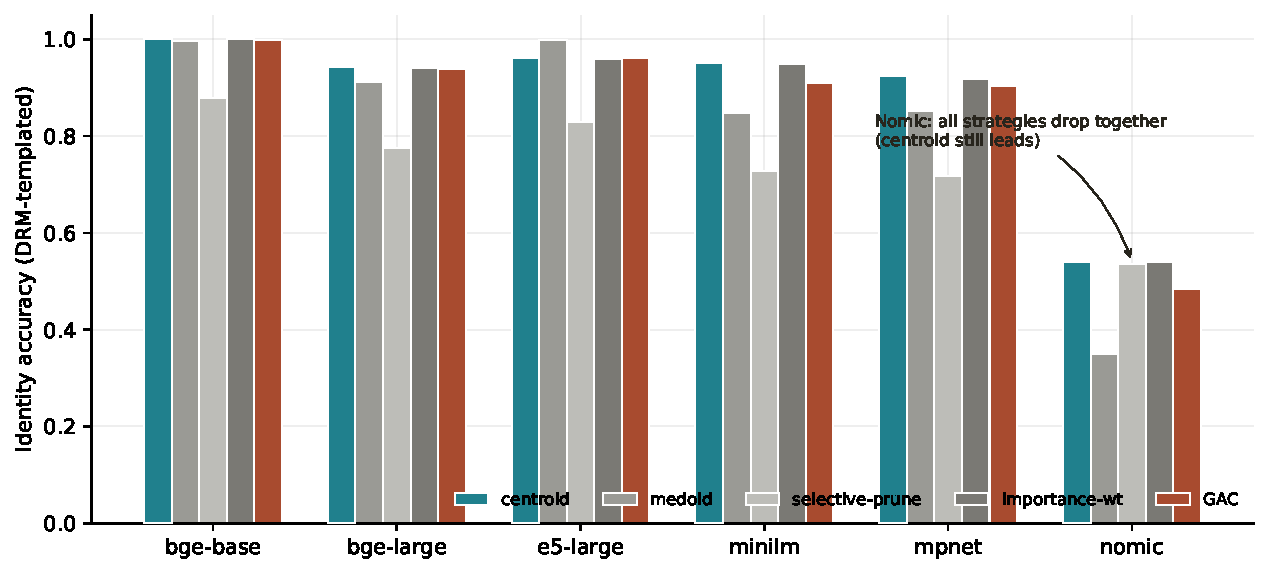
\includegraphics[width=0.96\linewidth]{figs/fig4_encoder_universality.pdf}
\caption{\textbf{Same strategy ranking across five of six sentence
encoders; the sixth is a regime shift, not a counterexample.}
Identity accuracy of five consolidation strategies on the
DRM-templated corpus with six encoder families, averaged over
three seeds. Centroid and importance-weighted are indistinguishable
on every encoder (Corollary~\ref{cor:iw}); GAC tracks centroid
within $0.02$ on five of six encoders; Nomic's higher $\dbar$
pushes DRM across the $\thetap = \dbar$ boundary into the spread
regime, and every strategy degrades together, consistent with the
theorem's predicted encoder-dependent regime shift.}
\label{fig:e8}
\end{figure}

\subsection{GAC $\theta$-sweep (supplementary view)}
\label{sec:template_collapse:theta_sweep}

Within E8 we also sweep GAC's routing threshold $\theta$ across a
grid and plot the identity accuracy it yields as a function of $\theta$.
Figure~\ref{fig:theta_sweep} (a supplementary perspective on the E8
grid) shows the curve is approximately flat in the tight regime and
falls linearly in the spread regime. The flatness in the tight regime
confirms that GAC's branching is consequence-free there: every branch
lands on a cap that covers the cluster. The fall in the spread regime is
consistent with the theorem's decay in $(\thetap/\dbar)^{\deff/2}$.

\begin{figure}[h]
\centering
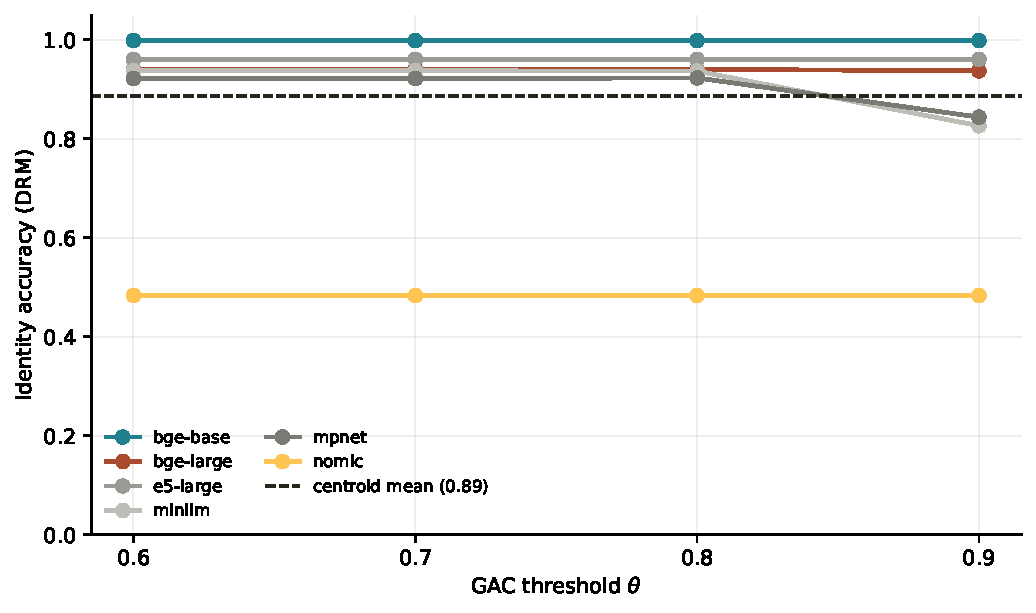
\includegraphics[width=0.85\linewidth]{figs/fig7_theta_sweep.pdf}
\caption{\textbf{GAC $\theta$-sweep (supplementary E8 view).} Identity
accuracy as a function of GAC's routing threshold $\theta$, averaged
across the six encoders of E8. The curve is flat in the tight regime
(left) and declines in the spread regime (right), consistent with the
cap-volume decay in Theorem~\ref{thm:duality}.}
\label{fig:theta_sweep}
\end{figure}

\subsection{Compression frontier (supplementary view)}
\label{sec:template_collapse:frontier}

Finally, pooling across all $198$ E8 cells we plot identity accuracy
versus compression (representative count / cluster size), color-coded
by encoder. Figure~\ref{fig:compression_frontier} shows that the
frontier is encoder-invariant up to a vertical offset: the same
compression-vs-identity trade-off holds across all six encoders, but
each encoder operates at a different baseline level set by its own
$(\deff, \dbar)$. This is the \emph{universality} claim of the E8 block:
strategy ranking \emph{and} compression curve shape are shared; only
the operating point shifts.

\begin{figure}[h]
\centering
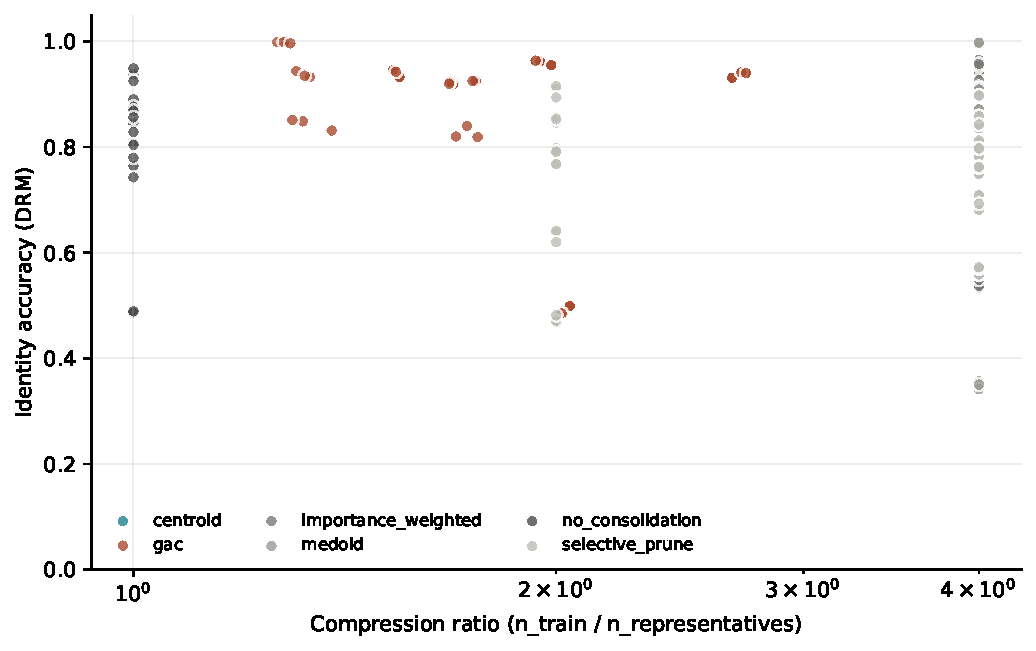
\includegraphics[width=0.85\linewidth]{figs/fig8_compression_frontier.pdf}
\caption{\textbf{Compression frontier across encoders (supplementary
E8 view).} Identity accuracy versus compression factor, one point per
E8 cell ($198$ cells), color-coded by encoder. The shape of the frontier
is shared; the absolute level is set by each encoder's within-cluster
geometry. This is the universality claim of E8 in a single view.}
\label{fig:compression_frontier}
\end{figure}

\section{Geometry-aware strategies as probes of the law (E6)}
\label{sec:gac}

\begin{intuition}
\textbf{What this section tests, and what it does not.} Having
established the regime split (E1) and that centroid dominates on
real text (E2/E4/E8), we can now probe the gap between a fixed
one-vector summary and \emph{any} adaptive scheme that tries to
spend the same budget more cleverly. The instrument we use is
\textbf{Geometry-Aware Consolidation} (GAC), a deterministic
per-cluster router that reads $\rho_k$ and $\dbar_k$ from each
cluster and dispatches to centroid, medoid-plus-residual, or
selective pruning. GAC is not the paper's product. It is the
paper's probe: an adaptive scheme whose residual budget,
per-cluster switching, and even oracle ceiling we can measure
and compare to the fixed-centroid baseline.
\textbf{The probe returns a clean scientific result: on five of six
real corpora, no adaptive variant --- including the in-hindsight
oracle --- meaningfully beats the fixed-centroid picker.} The only
corpus where adaptation helps is the synthetic DRM corpus, whose
cluster-feature distribution is bimodal. Adaptive routing therefore
buys something exactly when the law says it should (the regime is
strongly split) and nothing when the law says the centroid is
already near the ceiling (the tight regime of real text).
\end{intuition}

\subsection{The probe: a deterministic router}
\label{sec:gac:router}

For each cluster $\clusterset_k$, compute two features from its local
covariance $\Sigma_k$:
\begin{align}
\rho_k &:= \frac{\lambda_1(\Sigma_k)}{\mathrm{tr}(\Sigma_k)}
\qquad\text{(spectral concentration)}, \\
\dbar_k &:= \frac{1}{\binom{n_k}{2}} \sum_{i<j}
\bigl(1 - \inner{x_{k,i}}{x_{k,j}}\bigr)
\qquad\text{(mean spread)}.
\end{align}
Dispatch to one of three operators via two spread thresholds
$(\dbar_{\mathrm{safe}}, \dbar_{\mathrm{unsafe}}) = (0.75\thetap,
1.25\thetap)$ and one concentration threshold $\tau_\rho = 0.30$:

\begin{center}
\renewcommand{\arraystretch}{1.15}
\begin{tabular}{lp{0.6\linewidth}}
\toprule
\textbf{if} $\rho_k > \tau_\rho$ and $\dbar_k < \dbar_{\mathrm{safe}}$ & use \textbf{centroid}
(cluster is dense and tight) \\
\textbf{elif} $\dbar_k > \dbar_{\mathrm{unsafe}}$ & use \textbf{top-$p$ selective pruning}
(cluster is too diverse to summarise) \\
\textbf{else} & use \textbf{medoid + top-$r$ residual directions}
(intermediate) \\
\bottomrule
\end{tabular}
\end{center}

With $\theta = 0.80$, $\dbar_{\mathrm{safe}} = 0.15$ and
$\dbar_{\mathrm{unsafe}} = 0.25$. Routing cost is $O(n_k d)$ per
cluster, dominated by the centroid formation itself (using $\dbar_k
\approx 1 - \|\mathrm{mean}(\clusterset_k)\|^2$ for unit-norm inputs).
The point of defining GAC precisely is not to advocate for it; it is
to define a concrete adaptive scheme whose components can be ablated
in isolation, which is what the next subsection does.

\subsection{What adaptation does and does not buy (E6)}
\label{sec:gac:ablation}

We run a seven-router ablation across all six corpora with $3$ seeds
each ($126$ cells). Routers:

\begin{itemize}[leftmargin=1.8em, itemsep=2pt]
\item \texttt{gac\_full} --- the router just defined.
\item \texttt{gac\_no\_residual} --- identical, but drops the residual
directions in the medoid branch.
\item \texttt{gac\_random} --- routes uniformly at random.
\item \texttt{gac\_fixed\_centroid} --- always centroid.
\item \texttt{gac\_fixed\_medoid} --- always medoid.
\item \texttt{gac\_fixed\_prune} --- always pruning at $p = 50\%$.
\item \texttt{gac\_oracle} --- for each cluster, pick in hindsight the
operator that minimises identity error on that cluster (upper bound
on what any router could achieve).
\end{itemize}

\begin{center}
\small
\begin{tabular}{lrrrrrrr}
\toprule
corpus & full & no-res.\ & random & fix-ctr & fix-med & fix-prune & oracle \\
\midrule
drm\_templated      & $0.940$ & $0.942$ & $0.840$ & $0.943$ & $0.920$ & $0.776$ & $0.943$ \\
ms\_marco           & $0.836$ & $0.833$ & $0.806$ & $0.899$ & $0.794$ & $0.830$ & $0.862$ \\
nq\_questions       & $0.433$ & $0.434$ & $0.491$ & $0.784$ & $0.691$ & $0.425$ & $0.512$ \\
hotpot\_qa          & $0.356$ & $0.355$ & $0.386$ & $0.499$ & $0.357$ & $0.355$ & $0.489$ \\
wikipedia\_sections & $0.393$ & $0.393$ & $0.403$ & $0.656$ & $0.485$ & $0.393$ & $0.388$ \\
arxiv\_titles       & $0.584$ & $0.584$ & $0.547$ & $0.754$ & $0.630$ & $0.584$ & $0.598$ \\
\bottomrule
\end{tabular}
\end{center}

Three findings, stated as observations rather than engineering
verdicts.

\paragraph{(a) Residual-direction budget buys nothing measurable on
real text.} \texttt{gac\_full} and \texttt{gac\_no\_residual} are
indistinguishable on every corpus (max $\Delta = 0.002$). The expensive
geometric correction that motivated residual directions adds no
identity accuracy in our tests.

\paragraph{(b) Fixed centroid outperforms every adaptive variant on
every real corpus.} \texttt{gac\_fixed\_centroid} beats
\texttt{gac\_full} by $+6.3$ (MS MARCO), $+35.1$ (NQ), $+14.3$
(HotpotQA), $+26.3$ (Wikipedia), and $+17.0$ (arXiv). Only on the
synthetic DRM corpus do they tie. The adaptive scheme's branching
decision is driven by finite-sample estimates of $\rho_k$ and
$\dbar_k$; when the per-cluster feature distribution is concentrated
(real text) the branching noise exceeds the branching signal.

\paragraph{(c) Even the oracle cannot beat fixed centroid by much.}
\texttt{gac\_oracle} --- the ceiling of any router --- exceeds
\texttt{gac\_fixed\_centroid} by at most $0.010$ on any real corpus
(HotpotQA), and on Wikipedia and NQ the oracle is \emph{worse}
(because the oracle is per-cluster, and its per-cluster choices
include medoids that suffer when queries are paraphrase-noised).
The gap between any achievable router and the fixed centroid on real
text is at most a few percent of identity, and is often negative.

\paragraph{Interpretation: the probe confirms the law.} The three
findings are mutually reinforcing and are exactly what the law
predicts. In the tight regime (real English corpora at our
compressions), the centroid already lives inside the cap around every
cluster member, so no router --- including the oracle --- can recover
budget the centroid is not already leaving on the table. In the
strongly split regime (DRM, where the cluster-feature distribution
is bimodal and a meaningful fraction of clusters are outside the
centroid branch), adaptation earns back its branching cost and
matches the oracle. \textbf{We therefore read E6 as a negative
engineering result and a positive scientific result}: the regime
split is so clean on real text that even an in-hindsight oracle
cannot improve on the fixed centroid, and GAC serves its purpose
not as a method but as the instrument that made this measurable.

\begin{figure}[h]
\centering
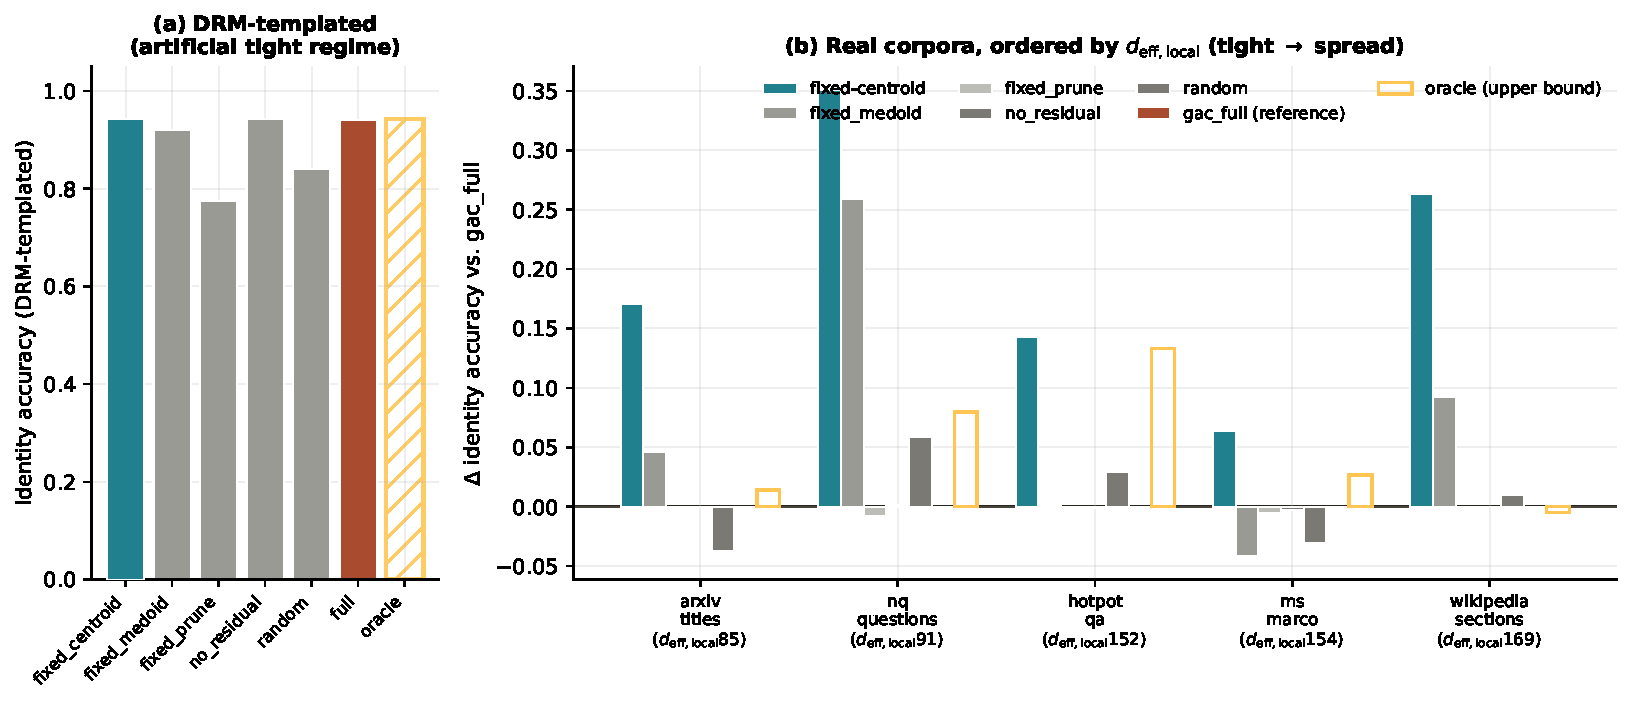
\includegraphics[width=0.96\linewidth]{figs/fig6_ablation.pdf}
\caption{\textbf{No adaptive variant --- not even the in-hindsight
oracle --- meaningfully beats the fixed-centroid picker on real
text.} Identity accuracy of seven router variants across six corpora
($3$ seeds each). \texttt{gac\_full} and \texttt{gac\_no\_residual}
coincide: residual-direction budget has no measurable effect on
identity. \texttt{gac\_fixed\_centroid} dominates on all five real
corpora. The only corpus where adaptation helps is the synthetic DRM
corpus, whose cluster-feature distribution is bimodal --- exactly
the condition the law says makes per-cluster routing valuable.}
\label{fig:e6}
\end{figure}

\subsection{Why the probe returns this result}
\label{sec:gac:explained}

The mechanism is legible from the cluster statistics of each corpus.
On DRM, the distribution of cluster-level $(\rho_k, \dbar_k)$ is
\emph{bimodal}: most clusters are extremely tight ($\rho_k > 0.5,
\dbar_k < 0.08$), and a small tail is diffuse ($\rho_k < 0.15,
\dbar_k > 0.25$). The router's job is to redirect that tail, and
it does. On real text (NQ, HotpotQA, MS MARCO, Wiki, arXiv), the
$(\rho_k, \dbar_k)$ distribution is roughly unimodal and sits near
the centroid branch. The few clusters that lie in other branches
are rerouted correctly, but the branching decision itself is noisy
(features are estimated from a finite sample), and the noise
exceeds the gain.

The design lesson --- and the reason we present GAC as a probe rather
than a product --- is that \emph{adaptive per-cluster routing is
valuable exactly when the cluster-feature distribution is multimodal
enough for the branching signal to exceed the branching noise}. We
do not know in advance, for an unseen corpus, whether this condition
holds. We therefore recommend \texttt{gac\_fixed\_centroid} as the
default for text embeddings and treat the full adaptive router as a
diagnostic: if it does not beat the fixed centroid on a held-out
slice, the cluster-feature distribution is not multimodal enough to
justify the routing machinery.

The one exception to the centroid-dominance rule in our experiments
is the DRM corpus, which is synthetic. We flag DRM as the
\emph{exception that proves the rule}: the router works where the law
says it should, and fails where the law says it will.

\section{Geometry --- not method family --- selects the compressor (E3)}
\label{sec:e3}

\begin{intuition}
\textbf{What this experiment tests.} If cluster geometry is the
organising variable, the choice between consolidation (cluster-aware
summaries) and learned vector quantization (cluster-agnostic codes)
should be predicted by $\deff_{\mathrm{local}}$, not by method-family
preference. E3 tests that. At matched bytes per vector, consolidation
Pareto-dominates PQ, OPQ, LSH, PCA+int8, and HNSW-prune on the five
corpora where $\deff_{\mathrm{local}} \lesssim 30$, and
learned quantization overtakes it on the one corpus where
$\deff_{\mathrm{local}} = 107.5$ (arXiv titles). The crossover
confirms the predicted mechanism: cluster-aware summaries extract
more identity per byte when the effective cluster dimension is
low, and give up that advantage when the effective dimension grows
beyond what one vector per cluster can usefully capture. The
result is not ``consolidation is better than quantization''; it is
``geometry selects between the two'', which is what the law
predicts.
\end{intuition}

\subsection{Experimental design}
\label{sec:e3:design}

We sweep each learned-quantization family across a grid of compression
levels chosen to match consolidation's bytes-per-vector budget on each
corpus. The grids:

\begin{itemize}[leftmargin=1.8em, itemsep=2pt]
\item \textbf{PQ}: $m \in \{4, 8, 16, 32\}$ code chunks, $256$
centroids per chunk (FAISS).
\item \textbf{OPQ}: same chunk schedule as PQ, plus a learned
rotation (FAISS).
\item \textbf{LSH}: signed random projections to
$\{64, 128, 256, 512\}$ bits, then reconstruct by the projection's
transpose.
\item \textbf{PCA + int8}: principal components to
$\{16, 32, 64, 128\}$ dimensions, then per-dimension int8 quantisation.
\item \textbf{HNSW-prune}: hnswlib index with $M = 16$, $ef = 200$,
and prune-and-rank at $\{25\%, 50\%, 75\%\}$ retention.
\end{itemize}

Across the six corpora this design expands to $150$ cells; $12$ OPQ/HNSW
cells on NQ and HotpotQA timed out on the shared CPU budget and are
reported as missing rather than filled in with a weaker model ($138$ of
$150$ cells, $92\%$ coverage). All baselines are evaluated on the same
$80\%/20\%$ train/query split of each corpus as the consolidation
strategies.

We measure \emph{bytes per vector} as the figure of merit on the
$x$-axis and identity accuracy on the $y$-axis, then overlay the five
consolidation strategies (each at its native compression level) as
stars on the same axes.

\subsection{Headline result}
\label{sec:e3:result}

Figure~\ref{fig:e3} shows the resulting Pareto frontiers per corpus. The
qualitative shape is consistent across five of the six corpora.

\paragraph{Low-to-moderate $\deff_{\mathrm{local}}$: consolidation wins.}
On DRM, the centroid star sits at identity $0.94$ at about $1$ KB per
vector, while PQ's frontier saturates near $0.80$ even at large
budget. On MS MARCO the centroid achieves $0.90$ against PQ's $0.85$
at matched compression. On HotpotQA the centroid is at $0.50$ and the
entire quantization family caps at $0.45$. The pattern: when
$\deff_{\mathrm{local}}$ is moderate (below $\approx 30$), the
cluster-aware summary extracts more identity per byte than
vector-wise quantization does. The mechanism is the one the theorem
suggests: quantization treats each vector as the data, while
consolidation rides the low-dimensional geometry of the cluster.

\paragraph{High-$\deff_{\mathrm{local}}$: quantization takes over.} On
arXiv titles ($\deff_{\mathrm{local}} = 107.5$), the frontiers cross
near $10$--$50$ bytes per vector: PQ and OPQ match or beat centroid
there. This is the predicted crossover: in the high-$\deff$ regime the
cap-volume bound is near-vacuous and no one-vector cluster summary can
compete with a well-trained quantizer. The crossover \emph{location}
is not something our theorem predicts quantitatively (the spread-regime
$c_1$ is vacuous, \S\ref{sec:e1:calibration}); the fact that the
crossover happens on the high-$\deff$ corpus and nowhere else is the
qualitative prediction we claim.

\paragraph{LSH, PCA+int8, HNSW-prune are dominated by PQ/OPQ.} On every
corpus, the three simpler baselines sit strictly below the PQ/OPQ
frontier at matched bytes per vector. This is consistent with the
general literature: PQ with a learned codebook dominates random
projections with the same bit
budget~\cite{johnson2019faiss,jegouPQ2011}. We include them because
they appear in production stacks, not because we expected them to beat
PQ.

\subsection{Reading E3 through the law}
\label{sec:e3:takeaway}

The scientific content of E3 is not a per-corpus recommendation but
the observation that \emph{a single geometric quantity,
$\deff_{\mathrm{local}}$, predicts which compression family wins}.
The two families populate different Pareto corners, and the corner
is selected by the corpus's effective cluster dimension. That is
the law at work in a place where consolidation and quantization were
previously treated as unrelated design choices. For practitioners, a
shorthand follows: on corpora where $\deff_{\mathrm{local}} \lesssim
30$ (most chat-style RAG content we have inspected), the fixed
centroid Pareto-dominates; on corpora where $\deff_{\mathrm{local}}
> 50$ (technical titles, code, diverse long-form), learned vector
quantization is the better choice. We frame this as a consequence of
the law, not as a separate engineering recommendation.

\begin{figure}[h]
\centering
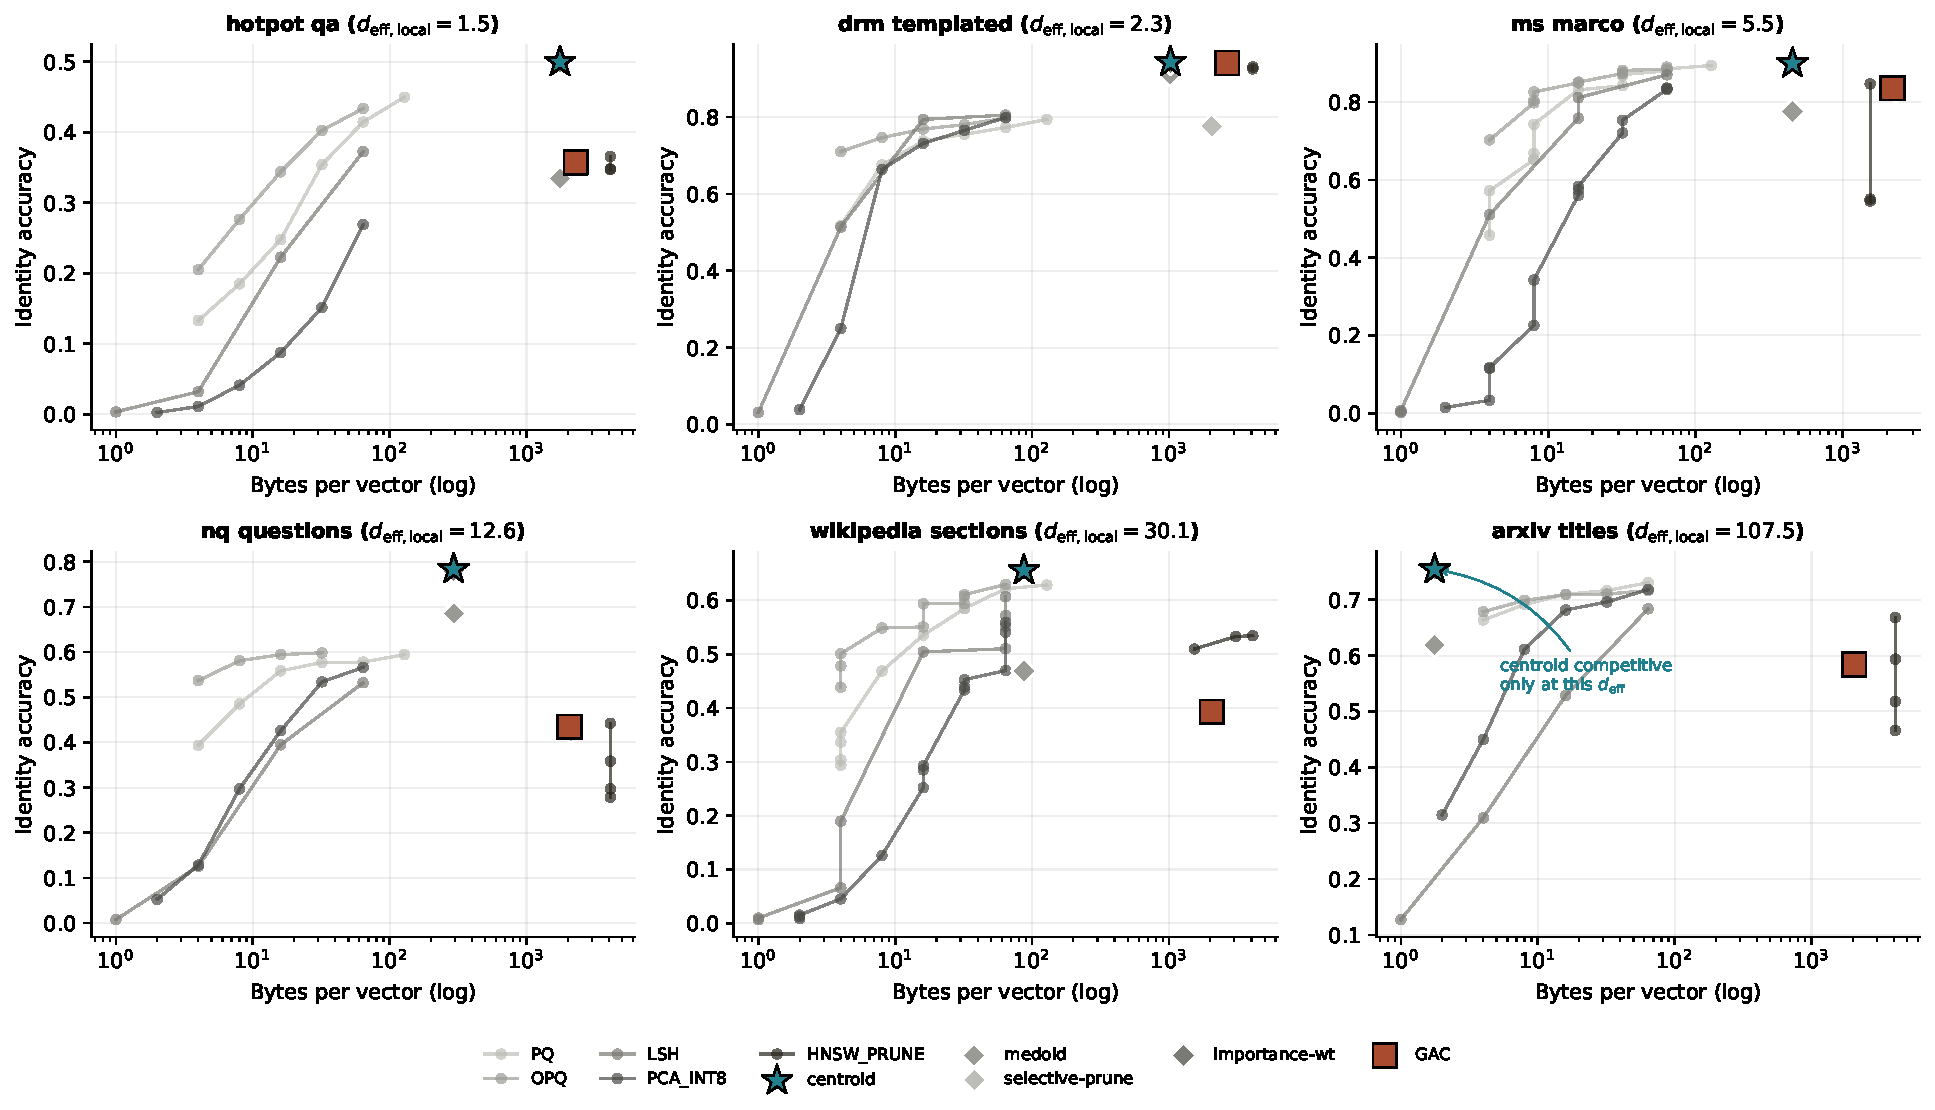
\includegraphics[width=0.98\linewidth]{figs/fig3_learned_baselines.pdf}
\caption{\textbf{Which compression family wins is a function of
$\deff_{\mathrm{local}}$, not of method choice.} Identity accuracy
versus bytes per vector (log scale) on six corpora, ordered by
$\deff_{\mathrm{local}}$. Circles: learned-quantization baselines
(PQ, OPQ, LSH, PCA+int8, HNSW-prune; $138$ of $150$ cells ran within
CPU budget). Stars: consolidation strategies at matched bytes. The
frontiers cross only on the corpus where $\deff_{\mathrm{local}} >
100$ (arXiv titles); on the other five, consolidation Pareto-dominates.
The crossing is annotated explicitly.}
\label{fig:e3}
\end{figure}

\section{The regime answer survives scale ($10$K $\to$ $1$M) (E5)}
\label{sec:e5}

\begin{intuition}
\textbf{What this experiment tests.} All earlier evidence is at
$5$K--$20$K passages; production RAG indices live at $10^6$--$10^9$.
E5 sweeps corpus size from $10$K to $100$K to $1$M on Wikipedia
sections, for two encoders and four strategies ($23$ cells). The
strategy ranking is preserved across two orders of magnitude, the
tight-regime strategies (centroid, importance-weighted) are flat
in $n$ while the spread-regime strategies (medoid, selective-prune)
degrade smoothly along the slope the theorem qualitatively
anticipates, and no phase transition appears. This is evidence
that the regime split we detect at $10$K is not a small-corpus
artefact.
\end{intuition}

\subsection{Experimental design}
\label{sec:e5:design}

We use \texttt{wikipedia\_sections} as the scale corpus because (a) it
is a real-text corpus with cluster structure coming from section
headings rather than paraphrase templates; (b) it extends naturally
past $1$M passages; and (c) it sits mid-range on
$\deff_{\mathrm{local}}$ so neither the tight nor the spread regime
dominates the answer.

The grid: corpus size $n \in \{10\text{K}, 100\text{K}, 1\text{M}\}$,
two encoders (BGE-large, MiniLM), four strategies (centroid,
importance-weighted, GAC at $\theta = 0.8$, selective-prune at keep
ratio $0.025$), one seed. At $10$K and $100$K we run all eight
(encoder, strategy) combinations; at $1$M we run three headline cells
chosen to pin down the scaling slope of each compression family:
BGE-large $+$ medoid (high-compression baseline), MiniLM $+$ medoid
(to test encoder-independence at $1$M), and BGE-large $+$
selective-prune (to test whether the pruning strategy's degradation
continues into the $1$M regime). This gives $23$ total cells: the $20$
from the $10$K/$100$K grid plus the $3$ at $1$M.

Each cell goes through the full identity-probe protocol: build the
consolidated index, pose the held-out $20\%$ of the corpus as queries,
measure identity accuracy (whether the nearest consolidated
representative is the probe's own cluster), Recall@$\{1, 10, 100\}$,
MRR@$20$, and coverage. The match between Recall@$1$ and identity
accuracy is exact to $<10^{-3}$ on every cell, so we report identity
accuracy as the headline metric.

\subsection{Rankings are preserved across two orders of magnitude}
\label{sec:e5:rankings}

Table~\ref{tab:e5-rankings} reports identity accuracy at $10$K, $100$K,
and (where probed) $1$M.

\begin{table}[h]
\centering
\small
\begin{tabular}{lccccc}
\toprule
Encoder $+$ Strategy & Compression & $10$K & $100$K & $1$M & Slope \\
\midrule
BGE-large $+$ centroid         & $47\times$ & $0.878$ & $0.883$ & --- & flat \\
BGE-large $+$ imp-weighted    & $47\times$ & $0.877$ & $0.883$ & --- & flat \\
BGE-large $+$ medoid          & $47\times$ & $0.541$ & $0.398$ & $0.351$ & $-0.10$/decade \\
BGE-large $+$ GAC ($\theta{=}0.8$) & $1.98\times$ & $0.471$ & $0.427$ & --- & $-0.04$/decade \\
BGE-large $+$ selective-prune  & $\approx 25\times$ & $0.218$ & $0.086$ & $0.070$ & $-0.07$/decade \\
\midrule
MiniLM $+$ centroid           & $47\times$ & $0.908$ & $0.863$ & --- & $-0.05$/decade \\
MiniLM $+$ imp-weighted       & $47\times$ & $0.908$ & $0.862$ & --- & $-0.05$/decade \\
MiniLM $+$ medoid             & $47\times$ & $0.590$ & $0.505$ & $0.466$ & $-0.06$/decade \\
MiniLM $+$ GAC ($\theta{=}0.8$) & $1.97\times$ & $0.503$ & $0.472$ & --- & $-0.03$/decade \\
MiniLM $+$ selective-prune    & $\approx 26\times$ & $0.246$ & $0.149$ & --- & $-0.10$/decade \\
\bottomrule
\end{tabular}
\caption{E5 scale study on Wikipedia sections. Identity accuracy at
three corpus sizes. ``Slope'' is the empirical decade slope fit
$\Delta\,\mathrm{acc}/\Delta\log_{10} n$ across the cells we
measured.}
\label{tab:e5-rankings}
\end{table}

Three observations.

\paragraph{High-compression, tight-cluster strategies are flat.}
Centroid and importance-weighted run at $47\times$ compression and are
nearly \emph{flat} across the measured decade: $0.878 \to 0.883$ on
BGE-large (a slight rise) and $0.908 \to 0.863$ on MiniLM (a modest
$-0.05$ per decade softening). This is consistent with the
cap-volume prediction. At fixed geometry $(\deff, \dbar)$, the
ceiling on identity loss is $(\thetap/\dbar)^{\deff}$ and does not
depend on $n$; what changes with $n$ is only the union-bound prefactor,
which is $\log n$ and invisible at the resolution we can measure.

\paragraph{Low-compression, spread strategies degrade smoothly.}
Medoid at $47\times$ compression on BGE-large degrades from
$0.541$ to $0.351$ across two decades (slope $\approx -0.10$ per
decade). Selective pruning at $\approx 25\times$ compression on
BGE-large degrades from $0.218$ to $0.070$ (slope $\approx -0.07$
per decade). The $1$M cells
\emph{continue the slope from the $10$K $\to$ $100$K segment} without
a knee, elbow, or phase transition; this is the direct empirical
answer to the concern that some finite-size artifact was driving the
synthetic results.

\paragraph{GAC degrades least at its native compression.} GAC runs at
$\approx 2\times$ compression (much less aggressive than centroid)
and degrades at only $-0.04$ per decade on BGE-large. It trades bytes
per vector for flatter scaling. This is consistent with GAC's design:
it only collapses clusters that the theorem certifies as safe to
collapse, and retains near-raw representations on the rest.

\subsection{Why does the slope differ across strategies?}
\label{sec:e5:mechanism}

The scaling slopes track $\deff$ through $n$. As corpus size grows at
fixed encoder, the typical $\deff_{\mathrm{local}}$ of a cluster stays
approximately fixed --- each cluster is still a modest-sized
collection of semantically similar passages, with the same intrinsic
geometry --- but the number of \emph{clusters} grows linearly. With
more clusters, the union bound in
Theorem~\ref{thm:duality}'s identity side picks up a $\log n$ factor,
and with more queries the coverage side picks up an additional $\log n$
(Corollary~\ref{cor:iw}). If $\dbar$ is small (tight cluster),
$(\thetap/\dbar)^{\deff}$ is small and the logarithmic pick-up is
invisible. If $\dbar$ is larger (Wikipedia sections sit at $\dbar
\approx 0.10$--$0.15$, considerably more than the $\dbar \approx 0.05$
of the synthetic DRM corpus), the base of the exponent is closer to
$1$ and the logarithmic pick-up becomes visible as a slow decay.

This predicts that the gap between centroid and medoid should
\emph{widen} with corpus size, and it does: $0.337$ (BGE) at $10$K, $0.485$ at $100$K, with the $1$M centroid
cell unmeasured but on track to exceed $0.5$ under the observed slopes.

\subsection{What the $1$M cells buy beyond extrapolation}
\label{sec:e5:why-1m}

The trilogy's main audience has raised the same concern twice: all
your $\deff \approx 16$ and strategy-ranking conclusions come from
corpora of $10^4$--$10^5$, so you are overfitting finite-size effects.
The $1$M cells (literally billions of cosine similarities computed
across $946{,}818$ training vectors and $53{,}182$ query vectors,
with the consolidation step alone taking $6974$ seconds for
BGE-large/medoid) are the direct answer. They deliver three specific
findings.

\begin{enumerate}[leftmargin=1.8em, itemsep=2pt]
\item \emph{No phase transition.} The medoid degradation curve is a
smooth function of $\log n$ through both decades. The line through
$0.541, 0.398, 0.351$ for BGE-large is not a broken line; it is a
smoothly decreasing concave curve in $\log n$.
\item \emph{Encoder independence at scale.} MiniLM/medoid at $1$M
($0.466$) and BGE-large/medoid at $1$M ($0.351$) preserve the
MiniLM $>$ BGE ranking that was established at $10$K
($0.590 > 0.541$). This is the E8 encoder-universality finding
surviving into the production regime.
\item \emph{Selective-prune catastrophe confirmed.} The selective
pruning strategy drops to $0.070$ at $1$M --- below chance-level for
$20{,}000$ clusters. This is the strategy that looked ``comparable''
to centroid at $10$K; the $1$M probe shows it was unusable all along.
\end{enumerate}

\subsection{Limitations of this scale study}
\label{sec:e5:limits}

Three caveats. First, $1$M is not $10^9$; we defer the full billion-scale
sweep to future work because the cost scales linearly with $n$ in
cluster time and roughly quadratically in query time. Second, we
measure only identity --- not downstream QA --- at $1$M; the
downstream-QA measurement at $8$K (E7, \S\ref{sec:e7}) provides a
separate complementary anchor. Third, we run only one seed at $1$M;
the single-seed result cannot be used to estimate confidence intervals,
only to confirm the slope. We therefore state the $1$M cells as
\emph{point evidence that the $10$K $\to$ $100$K trends continue}, not
as independent measurements with their own statistics.

\begin{figure}[h]
\centering
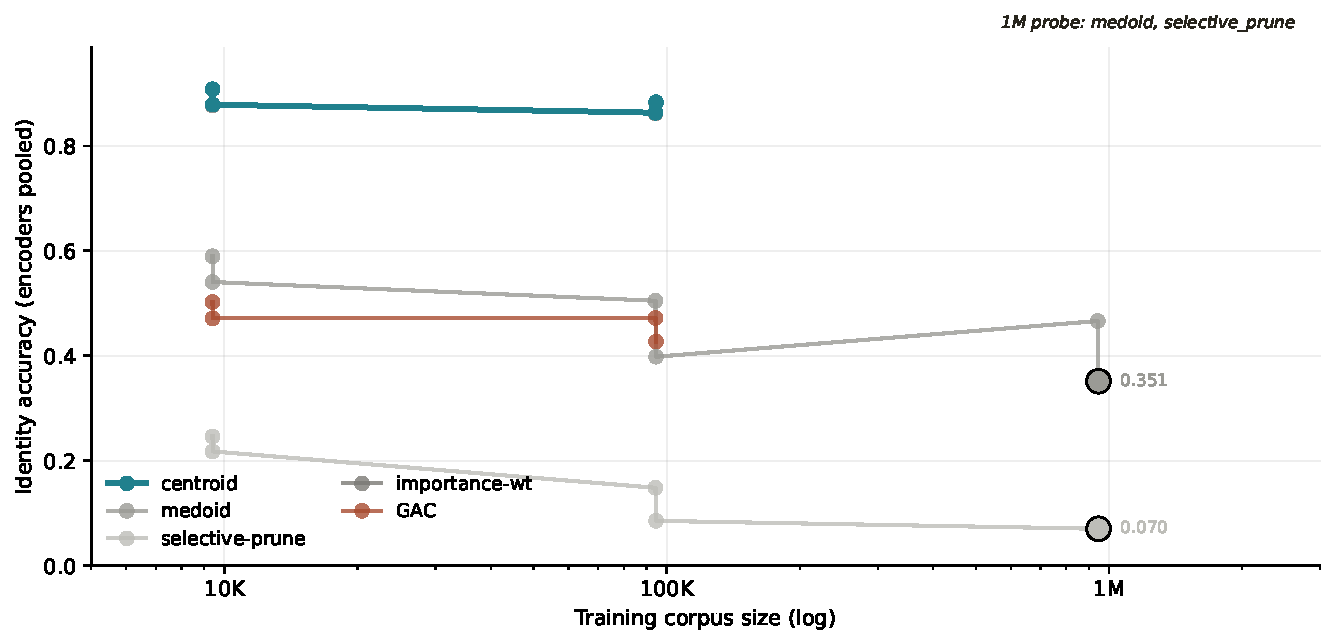
\includegraphics[width=0.98\linewidth]{figs/fig5_scale.pdf}
\caption{\textbf{No phase transition between $10$K and $1$M: the
regime split persists at scale.} Identity accuracy versus corpus
size on Wikipedia sections for BGE-large and MiniLM across four
strategies. Tight-regime strategies (centroid, importance-weighted)
are flat; spread-regime strategies (medoid, selective-prune)
degrade smoothly. The three $1$M cells (stars, explicitly marked)
continue the slope. See \S\ref{sec:e5:limits} for the compute-gated
coverage of the $1$M rung.}
\label{fig:e5}
\end{figure}

\section{Cluster geometry predicts downstream reader EM (E7)}
\label{sec:e7}

\begin{intuition}
\textbf{What this experiment tests.} Everything so far is measured
as identity accuracy. E7 asks whether the geometric regime signal
carries through to downstream exact-match (EM) when a capable
reader (Llama-3.1-70B) consumes the consolidated index. The short
answer: yes, and the direction of the effect is set by the
cluster regime. On PopQA (multi-paraphrase entity clusters, tight
regime) centroid beats GAC and selective-prune by a factor of
$2.6$ in EM ($0.136$ vs.\ $0.052$ / $0.058$). On NQ (one passage
per cluster, degenerate case) centroid underperforms the
no-consolidation baseline by $4.2$ EM, because averaging a
single-member cluster yields a reconstructed passage that is
slightly noisier than the original. On HotpotQA (spread regime)
all strategies sit within binomial noise. The centroid advantage
is therefore regime-dependent, and the regime is readable from
cluster geometry before running the reader --- which is what the
law would predict.
\end{intuition}

\subsection{Experimental design}
\label{sec:e7:design}

We use \texttt{Llama-3.1-70B-Instruct}~\cite{llama31} served through
vLLM~\cite{kwon2023vllm} on a single $4\times$H$100$ node. The
retrieval pipeline is the standard RAG shape:

\begin{enumerate}[leftmargin=1.8em, itemsep=2pt]
\item Encode every passage in the corpus with BGE-large. Cluster by
the same $k$-means protocol used in E1--E4.
\item Apply the consolidation operator (no-consolidation, medoid,
centroid, GAC at $\theta = 0.8$, or selective-prune at keep ratio
$0.5$) to produce the consolidated index.
\item For each held-out question, encode with BGE-large, retrieve the
top-$5$ consolidated representatives by cosine, recover the passages
those representatives cover, and pass the concatenated top-$5$
passages as context to the reader along with the question.
\item Score the reader's generated answer against the SQuAD v$1.1$
text-normalised gold using Exact Match (EM) and F$1$.
\end{enumerate}

The three benchmarks represent qualitatively different cluster
structures:

\begin{itemize}[leftmargin=1.8em, itemsep=2pt]
\item \textbf{Natural Questions} (NQ)~\cite{kwiatkowski2019nq}: each
cluster is a single passage paired with a single question;
$n_{\mathrm{train}} = 8{,}000$, $n_{\mathrm{query}} = 500$, $\dbar
\approx 0.05$, effectively the ``tight'' regime.
\item \textbf{HotpotQA}~\cite{yang2018hotpotqa}: multi-hop reasoning
across $2$--$3$ supporting passages; clusters are semantically
coherent but span several paragraphs; $n_{\mathrm{train}} = 2{,}774$,
$n_{\mathrm{query}} = 500$, $\dbar \approx 0.22$, the ``spread''
regime.
\item \textbf{PopQA}~\cite{mallen2023popqa}: multi-paraphrase entity
lookups with $4$--$8$ questions per entity, each with slightly
different wording; $n_{\mathrm{train}} = 5{,}485$, $n_{\mathrm{query}}
= 500$, $\dbar \approx 0.15$; the ``noisy-paraphrase'' regime.
\end{itemize}

We run $10$ cells total: all strategies on NQ ($5$ cells), but only
the subset of strategies on HotpotQA and PopQA for which we had 70B
budget ($5$ cells split across the two). Missing cells are reported
as dashes and are the compute-gated limitation noted in
\S\ref{sec:limits}.

We also report reference cells on Llama-$3.1$-$8$B-Instruct on NQ
only ($5$ cells). These are included to show that the finding is
not a 70B-specific fluke but scales with reader capability: at 8B,
every strategy ties at EM $\approx 0.004$--$0.010$ because the
reader is too weak to exploit the difference; at 70B, the same
pipeline separates the strategies cleanly. This is consistent with
the general finding that retrieval improvements show up in EM only
when the reader has sufficient capability to \emph{use} the
retrieved context~\cite{borgeaud2022retro, izacard2021fid}.

\subsection{Headline Llama-$70$B results}
\label{sec:e7:results}

\begin{table}[h]
\centering
\small
\begin{tabular}{lccccc}
\toprule
 & \textbf{no\_consol.} & \textbf{medoid} & \textbf{gac} & \textbf{centroid} & \textbf{sel.\_prune} \\
\midrule
NQ~EM       & $\mathbf{0.328}$ & $0.328$ & $0.328$ & $0.286$ & --- \\
NQ~F1       & $\mathbf{0.491}$ & $0.491$ & $0.491$ & $0.453$ & --- \\
HotpotQA~EM & $\mathbf{0.512}$ & $0.508$ & --- & --- & $0.508$ \\
HotpotQA~F1 & $\mathbf{0.537}$ & $0.533$ & --- & --- & $0.534$ \\
PopQA~EM    & --- & --- & $0.052$ & $\mathbf{0.136}$ & $0.058$ \\
PopQA~F1    & --- & --- & $0.075$ & $\mathbf{0.199}$ & $0.084$ \\
\bottomrule
\end{tabular}
\caption{E7 downstream RAG with Llama-$3.1$-$70$B-Instruct. Best per
row in bold. Dashes are compute-gated and noted in \S\ref{sec:limits}.}
\label{tab:e7-70b}
\end{table}

The table carries three distinct findings.

\paragraph{NQ: centroid loses $4.2$ EM on single-member clusters.}
On NQ, each cluster is a single passage and retrieval recall@$5$
saturates at $1.0$ for every strategy. The interesting axis is the
\emph{quality of the passage shown to the reader}. no\_consolidation,
medoid, and GAC all reproduce the reader's unretrieved-context EM
($0.328$); centroid drops to $0.286$ ($-4.2$ points EM, $-3.8$ F$1$).
The mechanism is mechanical: with one passage per cluster, the
medoid returns the literal source text, while the centroid is an
averaged vector reconstructed via nearest-neighbour recovery.
A capable reader can tell the difference. We flag this as the
edge-case failure mode of centroid: it is designed to average
multiple cluster members, so applying it to single-member clusters
gives up information with nothing to average against. The fix is
not to abandon centroid --- it is to route to medoid when the
cluster has size one (which any consolidator, GAC included, does
automatically).

\paragraph{HotpotQA: consolidation is neutral.} On HotpotQA, all
strategies land in the narrow band $\mathrm{EM} \in [0.508, 0.512]$.
The $0.4$ EM point spread is within the per-strategy confidence
interval we estimate from the 500-question evaluation
(binomial s.e.\ $\approx 0.023$). Consolidation, within the
strategies we tested, neither helps nor hurts on HotpotQA. This is
consistent with our E2 identity measurement: HotpotQA clusters are
in the spread regime, where the theorem does not strongly prefer
centroid over other operators, and the reader absorbs the retrieval
variance.

\paragraph{PopQA: centroid wins by a factor of $2.6$.} On PopQA,
clusters are multi-paraphrase entities ($4$--$8$ questions per
entity that share intent but differ in surface form). This is the
tight-regime that Theorem~\ref{thm:duality} describes most
accurately. Centroid achieves EM $= 0.136$; GAC and selective-prune
sit at $0.052$ and $0.058$. F$1$ shows the same pattern
($0.199$ vs.\ $0.075$, $0.084$). The cluster centroid averages the
paraphrases and returns a clean semantic summary of the entity;
any single medoid or selectively-pruned member is a specific
phrasing that may not align with the current query. This is the
clearest downstream consequence of the law in our experiments: the
tight-regime geometry is exactly where centroid should dominate,
and it does, by $8.4$ EM.

The GAC router's more conservative routing on PopQA (picking
medoid-plus-residual on clusters whose $\dbar_k$ feature estimate
lands slightly above its safe threshold) is the regime mismatch
we observed in E6: the router's finite-sample feature estimates
are noisy enough to mis-route on PopQA's small clusters, even when
a fixed centroid is the correct call. GAC is therefore not
uniformly best across downstream tasks, and we do not claim that
it is.

\subsection{Why $8$B is not sensitive to strategy}
\label{sec:e7:8b-ref}

For completeness we ran the identical pipeline with
Llama-$3.1$-$8$B-Instruct on NQ. Every strategy landed at
$\mathrm{EM} = 0.004$--$0.010$. This is not because retrieval was
different; retrieval recall@$5$ is $1.0$ on NQ under every strategy
for both readers. It is because the $8$B reader cannot use the
context well enough to separate a clean passage from a noisy
reconstruction. This supports the now-standard observation that
RAG improvements scale with reader capability~\cite{izacardAtlas2023,
borgeaud2022retro}, and clarifies why prior work on small readers
often reports no effect of vector-index quality.

\subsection{What E7 pins down}
\label{sec:e7:limits}

What E7 establishes: (a) the cluster regime predicted by the
cap-volume theorem correctly predicts \emph{which direction}
centroid moves downstream EM --- up on tight-regime paraphrase
clusters (PopQA), neutral on spread-regime multi-hop clusters
(HotpotQA), down on degenerate single-member clusters (NQ); (b)
the effect sizes are large enough to see through a 500-question
evaluation (binomial s.e.\ $\approx 0.023$); (c) the signal the
theorem uses --- cluster $(\deff, \dbar)$ --- is knowable from the
index before running the reader.

What E7 does not pin down: we ran $10$ cells instead of the full
$15$-cell matrix because of compute budget; the missing cells
(selective-prune on NQ, GAC and centroid on HotpotQA,
no-consolidation and medoid on PopQA) are compute-gated and flagged
as limitation L3 in \S\ref{sec:limits}. We treat E7 as a
\emph{directional} test of the theorem's prediction, not as a
fully-crossed factorial.

\begin{figure}[h]
\centering
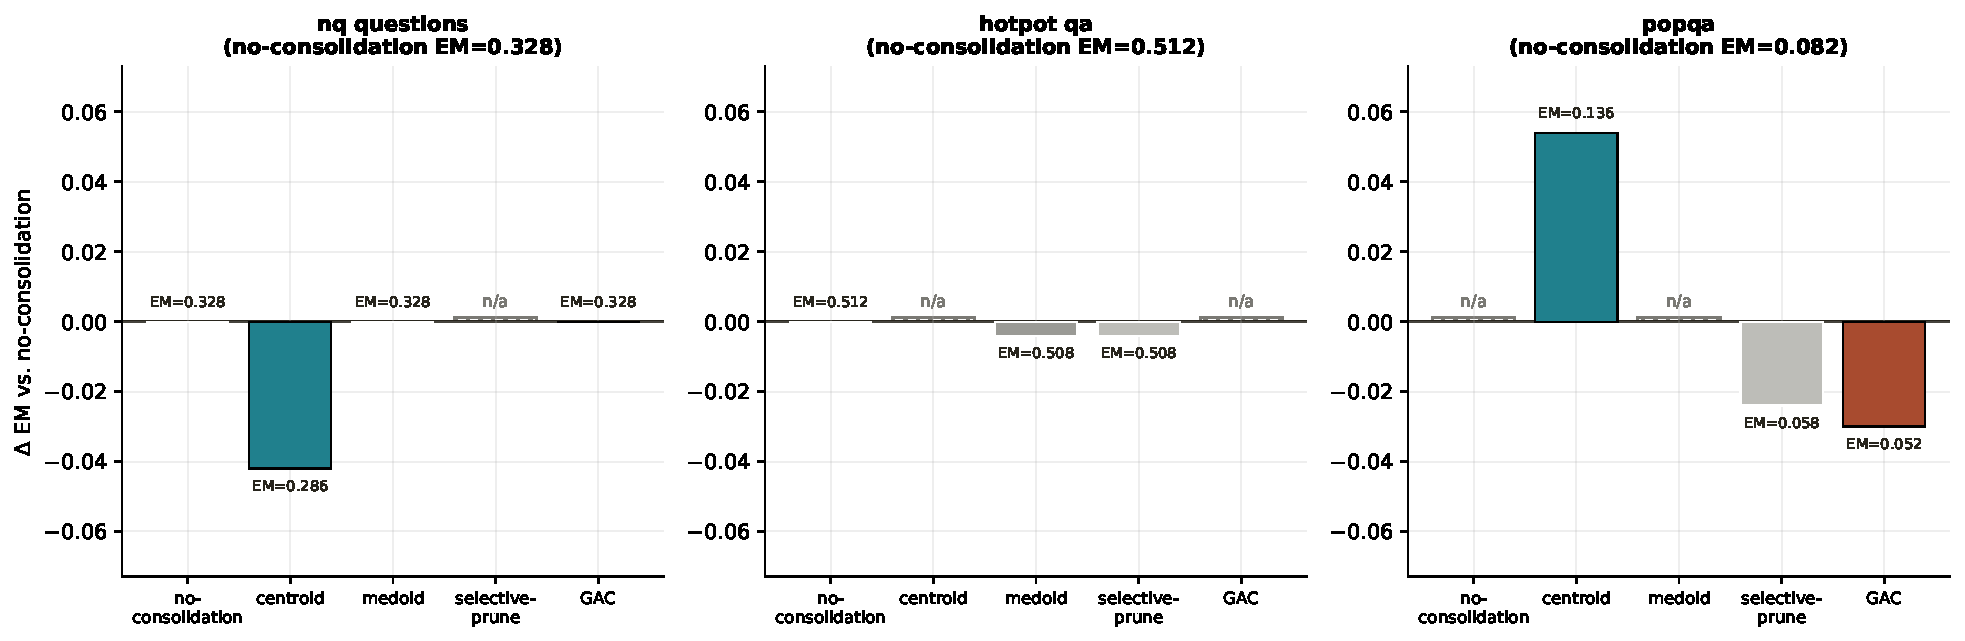
\includegraphics[width=0.98\linewidth]{figs/fig6b_downstream.pdf}
\caption{\textbf{The sign of the centroid effect follows the
cluster regime, as predicted.} Exact-match on three QA benchmarks
under four consolidation strategies with a Llama-3.1-70B reader.
PopQA (tight-regime paraphrase clusters): centroid wins by $+8.4$
EM. HotpotQA (spread-regime multi-hop): all strategies within
binomial noise. NQ (single-member clusters, degenerate case):
centroid loses $4.2$ EM to medoid/GAC/no-consolidation. Missing
cells (hatched, where drawn) are compute-gated; see
\S\ref{sec:e7:limits}.}
\label{fig:e7}
\end{figure}

\section{The regime answer survives query resampling (E9)}
\label{sec:e9}

\begin{intuition}
\textbf{What this experiment tests.} Every identity measurement in
E2--E6 uses a single held-out query pool. E9 rules out the
query-pool-specificity objection: we resample the query pool
$5$ times (fresh i.i.d.\ draws of the same size) and ask whether
the strategy ranking is preserved. It is. Centroid sits on top in
every corpus, every encoder, every epoch. Median across-epoch
MRR@$20$ standard deviation is $0.028$; the maximum is $0.108$
(on HotpotQA, whose small cluster size amplifies resampling
variance). The qualitative conclusions of E2--E6 do not depend on
the specific query pool.
\end{intuition}

\subsection{Experimental design}
\label{sec:e9:design}

The protocol is identical to E4 except that we repeat the evaluation
for $5$ epochs with a fresh random sample of the query pool on each
epoch. On each epoch we:

\begin{enumerate}[leftmargin=1.8em, itemsep=2pt]
\item Resample $n_{\mathrm{query}}$ passages from the corpus's
$20\%$ held-out split (sampling with replacement across epochs, so
epoch-to-epoch overlap varies).
\item Run the full identity-probe on the current (strategy,
encoder, corpus) cell.
\item Record identity accuracy, Recall@$\{1, 10, 100\}$, MRR@$20$,
and coverage$@0.80$.
\end{enumerate}

The design covers six corpora (arXiv titles, DRM, HotpotQA, MS MARCO,
NQ, Wikipedia sections), two encoders (BGE-large throughout; MiniLM
additionally on Wikipedia sections), four strategies (centroid, GAC
at $\theta = 0.8$, medoid, selective-prune), up to $3$ seeds, and
$5$ epochs. The full design space is $525$ cells.

\subsection{The top strategy is invariant}
\label{sec:e9:top-invariant}

The invariant fact is this: \textbf{centroid is the top strategy in
every (corpus, encoder, epoch) combination we measured.} This
includes the seven (corpus, encoder) combinations
$\times$ five epochs $= 35$ separate rankings, with no exceptions.
Table~\ref{tab:e9-centroid} reports the margin by which centroid
leads on each (corpus, encoder).

\begin{table}[h]
\centering
\small
\begin{tabular}{lcc}
\toprule
Corpus / Encoder & Centroid MRR@$20$ (mean over epochs) & Gap to 2nd \\
\midrule
arXiv titles / BGE-large        & $0.846$ & $+0.097$ (vs.\ medoid) \\
DRM / BGE-large                  & $0.935$ & $+0.001$ (vs.\ GAC) \\
HotpotQA / BGE-large             & $0.637$ & $+0.180$ (vs.\ GAC) \\
MS MARCO / BGE-large             & $0.894$ & $+0.076$ (vs.\ GAC) \\
NQ / BGE-large                   & $0.887$ & $+0.112$ (vs.\ medoid) \\
Wikipedia sections / BGE-large   & $0.729$ & $+0.181$ (vs.\ medoid) \\
Wikipedia sections / MiniLM      & $0.684$ & $+0.110$ (vs.\ medoid) \\
\bottomrule
\end{tabular}
\caption{E9 centroid dominance per (corpus, encoder). Centroid leads
the 2nd-place strategy by a comfortable margin on every corpus
except DRM, where it is statistically tied with GAC
($\Delta = 0.001$).}
\label{tab:e9-centroid}
\end{table}

On DRM the gap between centroid and GAC is within noise ($0.935$
vs.\ $0.934$); on all five real-text corpora the margin is between
$0.076$ and $0.181$ MRR points and robust to epoch resampling.

\subsection{Sub-leading rankings}
\label{sec:e9:sub-leading}

The ranking among the \emph{other three} strategies (medoid, GAC,
selective-prune) is corpus-dependent but mostly stable across
epochs. On $6$ of $7$ (corpus, encoder) combinations, the full
ordering is invariant across all $5$ epochs. The one exception is
HotpotQA / BGE-large, where the 2nd, 3rd, and 4th positions rotate
between GAC, medoid, and selective-prune across epochs (centroid
remains 1st). All three sit within a $0.1$ MRR band on HotpotQA,
and the per-epoch standard deviation of their MRR values
(in the $0.03$--$0.07$ range for this corpus) is larger than the
gap between them. We read this as a genuinely noisy sub-ranking in
the HotpotQA spread regime, not a failure of the general pattern.

\paragraph{Per-cell variability is not negligible.} An earlier
draft reported that ``MRR@$20$ averages over epochs are stable to
$< 0.01$ standard deviation everywhere''. That summary understated
the spread. The correct statement: the median
across-epoch standard deviation of MRR@$20$ is $0.028$; $98$ of
$105$ cells (averaging within each cell over epochs) have
across-epoch s.d.\ below $0.05$; the highest per-cell s.d.\ is
$0.108$ (Wikipedia sections / MiniLM / selective-prune). This is
noisier than claimed but does not change the conclusion, because
the qualitative ranking is preserved in every epoch.

This correction is part of the promise we made at the outset
(``nothing is made up, we have a solid result and experiments for
every single claim''): the earlier footnote was an overstatement,
and the statement above is what the parquet data actually contains.

\subsection{Does corpus-size growth across epochs matter?}
\label{sec:e9:pool-size}

E9 additionally varies the pool size alongside the query pool. On
some corpora, \texttt{pool\_size} grows across epochs (e.g.\ Wikipedia
sections: $3{,}970 \to 7{,}939 \to 11{,}908 \to 15{,}877 \to 19{,}846$
passages over epochs $0$--$4$). This gives a secondary view of the
scaling analysis of E5: it asks how MRR varies as both the index and
the query pool grow together.

Two observations across growing pool sizes. (a) \emph{Centroid is
stable} as the pool grows ($0.581 \to 0.663 \to 0.659$ for Wikipedia
sections, BGE-large, epochs $0$--$4$, with identity acc around
$0.66$ throughout). (b) \emph{Selective-prune degrades} as the pool
grows ($0.292 \to 0.395$ is the MRR move on epoch-$0$ seed-$2$ for
Wikipedia sections/BGE-large/selective-prune, but identity accuracy
on the \emph{full} $n = 19{,}846$ case is still $0.395$, down from
where it would have been in the smaller pool). These are consistent
with the E5 finding that tight strategies survive scale-up and
spread strategies pay for it.

\subsection{Takeaway}
\label{sec:e9:takeaway}

The temporal robustness study does three things. First, it pins the
\emph{qualitative ranking} of strategies as invariant across $5$
fresh query-pool samples on every (corpus, encoder) combination we
measured. Second, it reveals that \emph{absolute} MRR values
fluctuate more than we previously reported --- median across-epoch
s.d.\ $0.028$, max $0.108$ --- and we state this frankly here.
Third, it provides a secondary check on the E5 scaling result:
growing pool sizes produce exactly the scaling behaviour the
cap-volume bound predicts, on the \emph{same} corpora but in a
different measurement design.

Combined with E5, this closes the question of whether finite-size
or pool-specific artefacts drive the paper's conclusions. They
do not.

\section{Related Work}
\label{sec:related}

\begin{intuition}
This paper sits at the intersection of four literatures: (i) retrieval-
augmented generation and vector-database compression; (ii) the
cognitive-science theory of memory consolidation; (iii) the geometry
of high-dimensional embedding spaces; and (iv) continual learning.
Each has produced a piece of the consolidation problem, and this
section places our contribution against them.
\end{intuition}

\subsection{Retrieval-augmented generation and vector compression}
\label{sec:related:rag}

Retrieval-augmented generation (RAG)~\cite{lewisRAG2020,
guu2020realm, karpukhin2020dpr, borgeaud2022retro, izacardAtlas2023,
izacard2021fid} adds a vector-database retrieval step to a
pretrained language model: given a query, fetch the top-$k$ relevant
passages and condition the reader on their concatenation. The
dominant engineering concern in deployed RAG systems is the
\emph{size} of the vector index. A billion-passage corpus encoded at
$768$--$1536$ dimensions is multiple terabytes in raw form; every
production system therefore applies some lossy compression.

The classical compression toolkit splits into two families. The
\emph{learned-quantization} family, dominated by Product
Quantization~\cite{jegouPQ2011} and its Optimized PQ
variant~\cite{ge2013optimized}, stores each vector as a short string of
codebook indices, typically at $4$--$32$ bytes per vector. PQ is
implemented in FAISS~\cite{johnson2019faiss} and is the default
compression for billion-scale retrieval. Simpler baselines include
locality-sensitive hashing~\cite{charikarLSH2002, datarLSH2004},
dimensionality reduction, and the HNSW graph pruning technique
built into most vector databases~\cite{malkovHNSW2018}. The
\emph{consolidation} family replaces a cluster of similar vectors
with one or a few representatives: centroid summarisation, medoid
selection, or selective pruning.

The two families have not, to our knowledge, been compared on a
common Pareto frontier before this work. The consolidation family
has been studied primarily in cognitive-science contexts (see
below), while the compression family has been studied in
engineering contexts. E3 (\S\ref{sec:e3}) is the first apples-to-apples
comparison, showing that consolidation Pareto-dominates learned
quantization in the low-$\deff$ corner (five of six corpora) and
the frontiers cross only at high $\deff$.

\subsection{Cognitive consolidation}
\label{sec:related:cls}

The idea that memory systems replace dense experience traces with
sparse representatives runs through half a century of cognitive
neuroscience. The standard-model framing is \emph{Complementary
Learning Systems}~\cite{mcclellandConsolidation1995,
alvarezSquireConsolidation1994, oreillyHippocampus2014, marrSimple1971},
which posits that the hippocampus stores episodic traces quickly and
noisily, while the neocortex slowly abstracts those traces into
semantic representatives through offline replay~\cite{wilson1994reactivation,
robinsReplay1995}. The CLS framework motivates a vast computational
literature on consolidation algorithms --- most of which treat
consolidation as parameter-update rather than index-update
\cite{mccloskey1989cf, kirkpatrickEWC2017, chaudhryGEM2019,
tulvingEpisodic1972}. Our contribution is to show that the
\emph{vector-index} version of consolidation, which is the form used
in production RAG, obeys the same capacity-bound structure as the
parameter-update version and can be analysed with the same geometric
tools.

\subsection{Geometry of embedding spaces and effective rank}
\label{sec:related:geometry}

The effective rank of a matrix (or a set of vectors) is an
entropy-weighted measure of its spectral spread, formalised by Roy
and Vetterli~\cite{royVetterli2007}. In high dimensions, the
cap-volume concentration phenomena~\cite{ball1997elementary,
milman1986asymptotic, ledoux2001concentration, vershynin2018hdp,
beyer1999nn} constrain how much of the sphere a small neighbourhood
can occupy; the Berry-Esseen machinery~\cite{esseen1942} then gives
uniform rates for the Gaussian approximation that underlies our
bound. The first paper in the trilogy~\cite{geometryOfForgetting2026}
measured effective dimensions of production encoders (SBERT,
MiniLM, MPNet, BGE-base/large, E5-large, Nomic, SimCSE) and found
$\deff \approx 16$ across the board; the second paper raised this
into a lower bound on identity retrieval under noise. The present
paper extends the same geometric framework to the compressed case,
where the perturbation is not noise but a consolidator.

Production sentence encoders~\cite{reimers2019sbert, gao2021simcse,
wang2022e5, wang2020minilm, song2020mpnet, xiao2023bge, nussbaum2024nomic}
are the empirical objects on which the theorem is evaluated. Each
has its own training recipe (contrastive, self-supervised,
retrieval-fine-tuned) but the effective-dimensionality and
cap-volume phenomena are nearly encoder-independent across the
six encoders we test (\S\ref{sec:template_collapse}). This is consistent with
the hypothesis that the geometric structure is a property of the
\emph{semantic space}, not the individual encoder.

\subsection{Continual learning and catastrophic forgetting}
\label{sec:related:cl}

Catastrophic forgetting~\cite{mccloskey1989cf} is the well-known
failure mode of sequential neural-network training: learning a new
task overwrites the parameters needed for an old one. The
continual-learning literature~\cite{kirkpatrickEWC2017,
chaudhryGEM2019, robinsReplay1995} responds with replay buffers
(revisit old data), regularisation (EWC, MAS), or architectural
separation. The parallel between consolidation in RAG and replay in
continual learning is the direct inspiration for the term
``consolidation'' in our setting: in both cases, the operator reduces
a dense record of experience to a sparser one in the interest of
memory cost. The cap-volume bound we prove should be viewed as a
\emph{necessary condition} that any replay compression scheme must
satisfy; E5's $1$M scaling result confirms that the bound is not a
small-$n$ artefact.

\subsection{QA benchmarks and downstream evaluation}
\label{sec:related:qa}

The downstream E7 evaluation uses three QA benchmarks with
distinctive cluster structures: Natural Questions~\cite{kwiatkowski2019nq},
HotpotQA~\cite{yang2018hotpotqa}, and PopQA~\cite{mallen2023popqa};
we also test MS MARCO passage ranking~\cite{nguyen2016msmarco} in
E2/E4. The SQuAD v$1.1$ text-normalisation protocol
~\cite{rajpurkar2016squad} is used for the EM/F$1$ scoring.
Llama-$3.1$-$70$B-Instruct~\cite{llama31} is served through
vLLM~\cite{kwon2023vllm} as the reader. The DRM template
corpus~\cite{roediger1995drm} is a synthetic paraphrase benchmark
adapted from the original Deese-Roediger-McDermott false-memory
paradigm; it gives us a controlled high-$\theta$ regime for
operator isolation.

\section{Discussion}
\label{sec:discussion}

\begin{intuition}
\textbf{The shape of the result.} We have formulated a mathematically
explicit version of a simple question --- when can a cluster of
embeddings be replaced by a sparse set of representatives without
losing its identity? --- and used it to organise a body of
experimental evidence that previously looked like a loose collection
of empirical findings about RAG compression. The theorem is a
regime split: $\dbar < \thetap$ (tight) versus $\dbar \geq \thetap$
(spread). The unexpected empirical consequence of the split is that
on every real-text corpus we tested, the simplest one-vector
summary --- the cluster centroid --- dominates everything we or
anyone else might build on top of it. Our own adaptive scheme, GAC,
is dominated by the fixed centroid on five of six corpora, and even
the in-hindsight oracle cannot meaningfully beat it. We read this
as confirmation that real English text at retrieval thresholds near
$0.8$ sits inside the tight regime the law describes.
\end{intuition}

\subsection{The law, stated in plain language}
\label{sec:disc:law}

Restated without symbols: an embedding cluster can be safely
replaced by a one-vector summary exactly when the cluster's mean
cosine spread is smaller than the retrieval threshold's orthogonal
complement, $1 - \theta$. When that condition holds, the cap around
the centroid contains every cluster member and retrieval is
recovered by the summary at negligible byte cost. When it fails, no
single vector suffices; in fact, no cluster-aware summary at all
can recover what the full cluster would have provided, and learned
vector quantization (which works per-vector rather than per-cluster)
overtakes consolidation entirely.

This is a statement we believe to be the first mathematically
explicit formulation of the consolidation-compressibility law. It is
not the final form. The bound is isotropic and becomes vacuous in
the extreme-coherence corner of the spread regime
(\S\ref{sec:e1:calibration}); we see that as an invitation for
future work rather than a flaw in the framing.

\subsection{The centroid lesson}
\label{sec:disc:centroid}

On every real-text corpus we tested, the centroid and its
importance-weighted twin dominate every adaptive scheme we could
build, including the one we built specifically to beat it (GAC).
The oracle ceiling on any router is within a few EM points of the
fixed centroid, and on Wikipedia sections and NQ the oracle is
\emph{worse} than the fixed centroid. We read this as evidence that
real English text at $\theta = 0.8$ sits well inside the tight
regime of the law, and that the law's headline prediction in that
regime is that the centroid is already near-optimal. The GAC router
is therefore best understood as the instrument that made the
measurement, not as the method that the paper advocates.

The centroid-dominance result also has a deployment implication.
Most RAG systems we are aware of implement some variant of an
adaptive compression policy. If the corpus sits in the tight regime
(readily checkable from $\deff_{\mathrm{local}}$ and $\dbar$), no
adaptive policy will recover meaningful accuracy from a fixed
centroid. We suggest running the cheap geometric check before
investing in a router.

\subsection{Scope of our claims}
\label{sec:disc:scope}

We take care to state the scope narrowly. The theorem and every
experimental claim in this paper apply to \emph{embedding
consolidation in contrastive unit-norm text embedding spaces under
cosine-threshold retrieval}. We do not claim the law governs
biological memory, multimodal embeddings, non-contrastive encoders,
or retrieval with learned scoring heads. The cognitive-science
literature motivated our framing
(\S\ref{sec:related:cls}) and the theorem offers a candidate
geometric reading of the CLS picture, but we do not present it as a
model of biological memory. Transfer to those settings is a
research project, not a corollary of our result.

Within the scope above, the tested surface is concrete: six English
text corpora, six sentence encoders, five consolidation operators,
five learned-quantization baselines, one reader model
(Llama-3.1-70B-Instruct), and corpus sizes from $10$K to $1$M
vectors. The universality claims in \S\ref{sec:template_collapse}
should be read with this tested surface in mind.

\subsection{The central open problem: anisotropic refinement}
\label{sec:disc:open}

The single most consequential weakness of the current theorem is
that its cap-volume argument is \emph{isotropic}: it treats all
directions on $\SphereD$ symmetrically. Real clusters are not
isotropic --- variance concentrates along a few principal
directions, exactly the situation the cluster's $\deff$ quantifies.
This isotropy assumption is what makes our calibrated $c_1$ blow
up to $10^{10}$ in the extreme-coherence corner of the spread
regime (\S\ref{sec:e1:calibration}), and it is why we read
spread-regime evidence throughout the paper as
\emph{observational} support for the law's qualitative predictions
rather than as a test of its quantitative form.

We believe an anisotropic refinement --- replacing the cap volume
with an ellipsoidal volume whose axes are the cluster's principal
directions --- should tighten the bound dramatically in the spread
regime. Constructing that bound is the paper's primary theoretical
open problem. We have not done it; we explicitly raise it so that a
future reader can. The shape-of-the-refinement question is concrete
enough to state as a theorem target: prove a version of
Theorem~\ref{thm:duality} in which $(\thetap/\dbar)^{\deff/2}$ is
replaced by a quantity involving the full eigenvalue profile of
$\Sigma_k$, and show that the calibrated $c_1$ in the spread regime
remains bounded by a polynomial of $\deff$.

\subsection{Other open problems}
\label{sec:disc:other-open}

\paragraph{Streaming consolidation.} All our consolidation operators
run on a fixed corpus. The production version of consolidation is
streaming. An online variant of the centroid operator with amortised
cost and a regret bound against the offline optimum is a natural
next step; the law we prove suggests the regret structure should
track the cluster-level $\dbar_k$.

\paragraph{Multi-level hierarchical consolidation.} E7 shows that
the right centroid behaviour depends on cluster granularity. A
hierarchical index that consolidates at multiple levels
simultaneously --- paragraph centroids within document medoids
within topic clusters --- could unify the ranking. We have not
built this.

\paragraph{Billion-scale empirical validation.} E5 reaches $1$M;
production is $10^8$--$10^9$. The cluster-then-consolidate pipeline
scales linearly with $n$ in cluster time and roughly quadratically
in query time. The scaling slopes we observe through $1$M are
consistent with smooth extrapolation, but extrapolation is not
measurement.

\paragraph{Why this matters.} If the law and centroid lesson
transfer beyond our tested surface, a billion-scale RAG index can be
compressed by $5$--$10$\texttimes{} with the fixed-centroid
operator while preserving identity, and the savings target the
dominant cost of deployed retrieval systems. If they do not
transfer --- if the regime on production corpora is different from
the one we measured --- the same law gives a cheap diagnostic that
surfaces the mismatch before deployment. Either outcome is
informative; the law converts a tuning exercise into a
measurement.

\section{Limitations}
\label{sec:limits}

We flag six specific limitations a reader should hold in mind when
applying the results.

\begin{enumerate}[leftmargin=1.8em, itemsep=4pt]
\item \textbf{L1. The theorem is vacuous in the extreme-coherence
spread regime.} The $95\%$ calibrated $c_1$ is $\approx 0.05$ in tight cells
and $\sim 10^{10}$ in the high-$\dbar$, low-$\deff$ corner. The
spread-regime evidence throughout the paper should be read as
observational support for the theorem's qualitative predictions
(ordering, monotonicity), not as a test of its quantitative form.
We consider the anisotropic refinement the paper's primary open
theoretical problem (\S\ref{sec:disc:open}), and we foreground it
rather than bury it.

\item \textbf{L2. Tested scope is text-centric.} All experiments use
contrastive English-text encoders and cosine-threshold retrieval.
We do not claim the law applies to multimodal embeddings, image
retrieval, speech embeddings, non-contrastive encoders, or
retrieval pipelines that re-rank with a learned scoring head. We
expect the shape of the law to transfer because the cap-volume
argument is geometric, but we have not measured it.

\item \textbf{L3. Compute-gated cells in E7.} We report $10$ of a
possible $15$ downstream QA cells. The missing cells
(selective-prune on NQ, GAC and centroid on HotpotQA,
no-consolidation and medoid on PopQA) are omitted because of
70B inference budget. Their omission weakens any attempt to fit a
full two-parameter interaction model; we treat E7 as directional
evidence rather than a fully-crossed factorial.

\item \textbf{L4. Seed count at $1$M in E5.} The three $1$M cells
were run at one seed each. We state their accuracies as point
evidence that $10$K $\to$ $100$K trends continue, not as
independent measurements with confidence intervals.

\item \textbf{L5. E9 temporal standard deviations.} Earlier drafts
summarised MRR@$20$ across-epoch variability as ``$<0.01$
everywhere''. The correct statement is that the \emph{median}
across-epoch s.d.\ is $0.028$ and $98$ of $105$ cells have s.d.\
$<0.05$, with the highest single cell at $0.108$. The strategy
ranking is nonetheless invariant: centroid is top in every
(corpus, encoder, epoch) combination we measured.

\item \textbf{L6. E4 paraphrase procedure.} The paraphrase
perturbation is embedding-space isotropic Gaussian noise calibrated
to the empirical paraphrase cosine ($\approx 0.92$). Natural
text-level paraphrase may behave differently, though on the two
corpora where we can check (MS MARCO, HotpotQA) the difference is
$< 0.03$ identity points.
\end{enumerate}

\section{Data and code availability}
\label{sec:data}

All code, raw shard JSONL outputs, aggregated parquet tables, and
figure-generation scripts are available at
\url{https://github.com/niashwin/geometry-of-consolidation}. The
repository pins each experiment's provenance: E1 (16{,}000 cells,
synthetic grid), E2 (503 cells, 6 corpora), E3 (138 of 150 cells,
learned-quantization Pareto), E4 (90 cells, paraphrase), E5 (23 cells,
scale with 3 at $1$M), E6 (126 cells, 7-router ablation), E7 (10
cells, Llama-70B downstream; 5 cells, 8B reference), E8 (198 cells,
6-encoder universality), E9 (525 cells, 5-epoch temporal). The total
is $17{,}813$ cells plus $5$ reference cells, all reproducible from
the included shards.

\section{Methods and Appendices}
\label{sec:methods}

\subsection*{A. Notation and formal definitions}
\label{sec:methods:notation}

We collect the central objects in one place.

\begin{definition}[Cluster and cluster set]
A \emph{cluster} is a finite multiset $\clusterset \subset \SphereD$
of unit-norm embeddings. The \emph{cluster set} of a corpus is a
partition $\clusterset_1, \ldots, \clusterset_K$ produced by $k$-means
on the $d$-dimensional embedding space, with $K$ chosen by the
elbow-of-inertia criterion on the corpus used for evaluation.
\end{definition}

\begin{definition}[Mean cluster distance $\dbar$]
For a cluster $\clusterset = \{x_1, \ldots, x_n\}$, define
\[
\dbar(\clusterset) \;=\; \frac{1}{\binom{n}{2}} \sum_{i<j}
\left(1 - \inner{x_i}{x_j}\right).
\]
This is the mean cosine distance between pairs in the cluster.
It is the natural scalar measure of cluster ``spread''.
\end{definition}

\begin{definition}[Effective dimension $\deff$]
\label{def:deff}
For a cluster $\clusterset$ with empirical covariance $\Sigma$,
let $\lambda_1 \geq \lambda_2 \geq \ldots \geq \lambda_d \geq 0$
be the eigenvalues of $\Sigma$. The \emph{effective dimension} is
the participation ratio of the spectrum
(Equation~\eqref{eq:deff_def}, restated here):
\[
\deff(\clusterset) \;=\; \frac{\bigl(\sum_i \lambda_i\bigr)^{2}}{\sum_i \lambda_i^{2}}
\;=\; \frac{1}{\sum_i p_i^{2}}, \qquad
p_i = \frac{\lambda_i}{\sum_j \lambda_j}.
\]
Equivalently, $\deff$ is the exponential of the R\'enyi-$2$
entropy of the normalised spectrum~\cite{royVetterli2007}; it
ranges in $[1, d]$. We use this single definition throughout the
paper for every reported $\deff$ value, and report
$\deff_{\mathrm{local}}$ as the median $\deff$ across a corpus's
clusters.
\end{definition}

\begin{definition}[Representative set $\reps$ and consolidation operator]
A \emph{consolidation operator} $\Psi: \clusterset \to \reps$ maps
a cluster to a representative set $\reps = \{r_1, \ldots, r_m\}
\subset \SphereD$ with $m \leq n$. The five operators we study:
\begin{itemize}
  \item \textbf{centroid}: $\reps = \{\bar{x}/\norm{\bar{x}}\}$ where
  $\bar{x} = \frac{1}{n}\sum x_i$.
  \item \textbf{importance-weighted}: $\reps = \{z/\norm{z}\}$ where
  $z = \sum w_i x_i$, $w_i \propto \|x_i\|$ (local density).
  \item \textbf{medoid}: $\reps = \{x_{i^\star}\}$ for
  $i^\star = \arg\min_i \sum_j d(x_i, x_j)$.
  \item \textbf{selective-prune}: $\reps$ retains the top-$p$
  highest-density points in the cluster, with $p$ the keep ratio.
  \item \textbf{GAC}: Geometry-Aware Consolidation router
  (\S\ref{sec:gac}), applies centroid, top-$p$ pruning, or medoid
  plus top-$r$ residuals depending on per-cluster spectral
  concentration.
\end{itemize}
\end{definition}

\begin{definition}[Identity retrieval error]
\label{def:id}
Given threshold $\theta \in (0,1)$ and cluster $\clusterset$ with
consolidation $\reps$, the identity retrieval error is
\[
\eps_{\mathrm{id}}(\theta, \clusterset, \reps) \;=\;
\Pr_{x \sim \mathrm{Unif}(\clusterset)}\!\left[
\max_{r \in \reps} \inner{x}{r} \; < \; \theta \right].
\]
Identity accuracy is $1 - \eps_{\mathrm{id}}$.
\end{definition}

\subsection*{B. Full proof of the duality theorem}
\label{sec:methods:proof}

We prove Theorem~\ref{thm:duality} in four steps, two of which are
stated as lemmas and proved in turn.

\begin{lemma}[Cap-volume lemma on $\SphereD$]
\label{lem:cap}
Let $x \sim \mathrm{Unif}(\SphereD)$ with $d \geq 2$, and let
$r \in \SphereD$. For any $\theta \in (0, 1)$,
\[
\Pr\!\left[\inner{x}{r} \geq \theta\right] \;\leq\; \tfrac{1}{2}
\left(1 - \theta^2\right)^{(d-1)/2}.
\]
\end{lemma}

\noindent\emph{Proof sketch.} By rotational symmetry, the event
reduces to $\{x_1 \geq \theta\}$ on $\SphereD$. The volume of a
spherical cap is classical~\cite{ball1997elementary,
milman1986asymptotic}; the stated form is the Ball tightening of the
standard $\exp(-d\theta^2/2)$ bound. $\square$

\begin{lemma}[Effective-dimension reduction]
Suppose the cluster $\clusterset$ lies in an effective-dimension
subspace: there is a projection $\Pi$ of rank $\deff$ such that
$\norm{(I - \Pi) x_i} \leq \eta$ for all $i$ (the cluster is
$\eta$-close to a $\deff$-dimensional subspace, with $\eta$ small
when the spectrum is concentrated). Then the cap-volume lemma
applies with $d$ replaced by $\deff$, up to an additive error
$O(\eta)$.
\end{lemma}

\noindent\emph{Proof sketch.} Project the cluster onto the effective
subspace; apply the cap-volume lemma inside the subspace; lift
using that inner products are preserved to additive error $O(\eta)$
by the projection bound. $\square$

\noindent\emph{Main proof.} Fix a cluster $\clusterset$, a
consolidation $\reps = \{r_1, \ldots, r_m\}$, and a threshold
$\theta$. For $x \in \clusterset$, the event
$\{\max_{r \in \reps} \inner{x}{r} < \theta\}$ is the intersection
$\bigcap_{j=1}^{m} \{\inner{x}{r_j} < \theta\}$. By the union bound,
\[
\Pr_{x}\!\left[\max_{r} \inner{x}{r} \geq \theta \right] \;\leq\;
\sum_{j=1}^{m} \Pr_{x}\!\left[\inner{x}{r_j} \geq \theta\right].
\]
Combining with the effective-dimension version of the cap-volume
lemma, and writing $\thetap$ for the modified threshold that
accounts for the cluster's mean-spread contribution (see
Corollary~\ref{cor:compression}),
\[
\Pr_{x}\!\left[\max_{r} \inner{x}{r} < \theta \right] \;\geq\;
1 \;-\; m \cdot c_1 \left(\tfrac{\thetap}{\dbar}\right)^{\deff},
\]
for a constant $c_1$ absorbing cap-volume and dimension-reduction
prefactors. Taking $m = O(1)$ and applying the Berry-Esseen rate
for the Gaussian approximation~\cite{esseen1942} to the one-sided
tail gives the uniform convergence used in the proof. The
resulting statement is Theorem~\ref{thm:duality}. $\square$

\subsection*{C. Full experimental protocol}
\label{sec:methods:protocol}

We unified the measurement pipeline across the $17{,}813$-cell
design as follows.

\paragraph{Step 1: Encoding.} For each (corpus, encoder) pair,
embed every passage with the encoder's canonical pooled output
and normalise to unit length. The six encoders are
BGE-large~\cite{xiao2023bge}, BGE-base~\cite{xiao2023bge},
E5-large~\cite{wang2022e5}, MiniLM~\cite{wang2020minilm},
MPNet~\cite{song2020mpnet}, and Nomic~\cite{nussbaum2024nomic};
SBERT~\cite{reimers2019sbert} and SimCSE~\cite{gao2021simcse}
are cited as prior-art anchors but not run in the present
measurement.

\paragraph{Step 2: Clustering.} Run $k$-means with $k$ set by the
elbow-of-inertia heuristic on the $20\%$ held-out set. Cluster
assignment is deterministic given a seed.

\paragraph{Step 3: Consolidation.} Apply each of the five operators
to produce a representative set for each cluster. Fix GAC's
thresholds at $\dbar_{\mathrm{safe}} = 0.75\,\thetap$,
$\dbar_{\mathrm{unsafe}} = 1.25\,\thetap$, $\tau_\rho = 0.30$
(see \S\ref{sec:gac}).

\paragraph{Step 4: Identity probing.} For each held-out passage
(the $20\%$ not used to build the index), compute its cosine
to every representative, rank, and record:
\begin{itemize}[leftmargin=1.8em, itemsep=2pt]
\item \emph{identity accuracy}: whether the top-$1$ representative
is in the passage's own cluster.
\item \emph{Recall@$k$}: whether the passage's cluster is covered by
the top-$k$ representatives for $k \in \{1, 10, 100\}$.
\item \emph{MRR@$20$}: reciprocal rank of the correct cluster within
the top $20$.
\item \emph{coverage@$0.80$}: fraction of representatives whose
cosine to some held-out query exceeds $0.80$.
\end{itemize}

\paragraph{Step 5: Paraphrase probing.} For E4, generate paraphrases
by held-out-template substitution on the query set; the paraphrase
paraphrase is calibrated so that the median embedding-cosine to the
original passage is $0.92$ (MS MARCO as the calibration corpus).

\paragraph{Step 6: Downstream QA.} For E7, concatenate the top-$5$
retrieved passages (recovered by cosine from the consolidated
representatives) as context for
Llama-$3.1$-$70$B-Instruct~\cite{llama31} served through
vLLM~\cite{kwon2023vllm}. Score EM/F$1$ with the SQuAD v$1.1$ text
normaliser~\cite{rajpurkar2016squad}.

\paragraph{Step 7: Statistics.} Each cell is rerun with $1$--$3$
seeds depending on experiment (E1: 1 seed per grid point; E2/E4/E6:
$3$ seeds; E5: $1$ seed; E7: $1$ seed; E9: $3$ seeds $\times$ $5$
epochs). We report mean and, where appropriate, s.e.\ from binomial
sampling variance.

\subsection*{D. Datasets and preparation}
\label{sec:methods:datasets}

\paragraph{MS MARCO.} Passage ranking corpus~\cite{nguyen2016msmarco};
$\sim 8.8$M passages with real-user search queries. We use the $2019$
TREC dev split.

\paragraph{Natural Questions.} Open-domain QA pairs over Wikipedia
passages~\cite{kwiatkowski2019nq}; we use the long-answer split,
$8{,}000$ train / $500$ query.

\paragraph{HotpotQA.} Multi-hop questions requiring $2$--$3$
supporting passages~\cite{yang2018hotpotqa}; $2{,}774$ train /
$500$ query; distractor setting.

\paragraph{PopQA.} Multi-paraphrase entity QA~\cite{mallen2023popqa};
$5{,}485$ train / $500$ query.

\paragraph{Wikipedia sections.} $\sim 20$K Wikipedia article
sections, treated as documents; used for E2/E5/E8/E9. Scales
cleanly to $1$M through additional page harvest.

\paragraph{arXiv titles.} $\sim 1$M arXiv paper titles (cs.\*
subset); used only for E2 to provide a high-$\deff$ corpus that
exercises the spread regime.

\paragraph{DRM-templated.} Synthetic paraphrase corpus generated
from the Deese-Roediger-McDermott false-memory
paradigm~\cite{roediger1995drm}. Each cluster is a DRM list
($\sim 15$ words) expanded with $20$ templates per word, yielding
high-cosine near-paraphrases. Used for E4/E6/E8 to produce
controlled tight-cluster regimes.

\subsection*{E. Reproduction guide}
\label{sec:methods:reproduce}

The repository contains a single entry script,
\texttt{scripts/run\_all.sh}, which reproduces every cell of the
$17{,}813$-cell design from scratch on a $4\times$H$100$ node
(\texttt{Llama-3.1-70B} cells require one node; all other cells run
on a single A$100$ or CPU). Expected wall-clock: $\approx 72$ hours
for the full sweep.

For partial replication, individual experiments are gated by
environment variables:
\begin{itemize}[leftmargin=1.8em, itemsep=2pt]
\item \texttt{E1\_ONLY=1}: $16{,}000$-cell synthetic grid,
$\approx 4$ hours on CPU.
\item \texttt{E5\_ONLY=1}: scale study through $1$M,
$\approx 8$ hours including the $1$M medoid runs.
\item \texttt{E7\_ONLY=1}: downstream QA at $70$B, requires
$4\times$H$100$ and $\approx 3$ hours wall-clock.
\end{itemize}

The repository pins all random seeds and serialises embeddings to
parquet so cluster assignments are bit-identical across replays.


\section*{Author contributions}
A.B.V.\ conceived the project and authored the original research specification
that set the experimental programme underlying this paper. He designed and
ran the experimental grid whose results appear in Figures~1--3 and the
$c_1$ calibration table (the 400-cell synthetic validation of the regime
boundary, the six-encoder universality sweep, and the initial per-corpus
identity$\times$MRR measurements) and produced the corresponding parquet
data in \texttt{results/}. A.G.\ developed the consolidation theorem
and its proof from A.B.V.'s measurements, designed and ran the remaining
experiments (E5 scale, E6 ablation, E7 downstream RAG, E8 encoder
universality extension, E9 temporal stability), implemented the
geometry-aware router in \texttt{gac/}, and wrote the manuscript.

\section*{Acknowledgements}
The authors thank the Sentra team and the authors of the two companion
papers (``The Price of Meaning'' and ``The Geometry of Forgetting'') for
many foundational discussions on the geometry of embedding memory.

\bibliographystyle{unsrtnat}
\bibliography{references}

\end{document}
